%% Chapter 3 — Inside Containers
\setcounter{chapter}{2}
\chapter{Inside Containers}
\chaptersubtitle{Namespaces, cgroups, and overlayfs — building the box your model server ships in}

\begin{calloutbox}{tbbblue}{tbbbluefill}
{\normalsize\bfseries\color{tbbblue}Learning objectives}\par\vspace{3pt}
\begin{tbbitemize}
  \item Explain the sentence "a container is namespaces + cgroups + a layered filesystem around an ordinary process" — and defend the stronger claim that the kernel has no container object at all.
  \item Describe what each of the six classic namespaces virtualizes, and reason about the consequences of PID namespace semantics (PID 1 duties, signals, zombies) and NET namespace wiring (veth, bridges, ports).
  \item Use cgroups v2 through its filesystem interface: set CPU quotas and memory limits, read usage and events, and compute by hand what CPU throttling does to a request's latency.
  \item Narrate exactly what happens when a process exceeds memory.max — reclaim, OOM kill, SIGKILL, exit code 137 — and right-size memory limits for an inference server's real memory shape, with numbers.
  \item Explain how overlayfs assembles image layers into a root filesystem, demonstrate copy-up and whiteouts at a shell, and connect layer hygiene to image size, build time, and cold-start latency.
  \item Build a working container by hand with unshare, pivot\_root, /proc, and a cgroup — reading every command's output — and state precisely what Docker adds on top (next week's subject).
\end{tbbitemize}
\end{calloutbox}

\vspace{5.0pt}

\begin{calloutbox}{tbbteal}{tbbtealfill}
{\normalsize\bfseries\color{tbbteal}Key terms}\par\vspace{3pt}
namespace (PID · NET · MNT · UTS · IPC · USER) · unshare / setns · PID 1 · zombie reaping · veth pair · bridge · rootless containers · cgroups v2 · controller · cpu.max · throttling · cpu.weight · memory.max · memory.high · memory.events · OOM killer · exit code 137 · oom\_score\_adj · overlayfs · lowerdir / upperdir / merged · copy-up · whiteout · image layer · pivot\_root · chroot
\end{calloutbox}

\vspace{5.0pt}

\begin{calloutbox}{tbblightgray}{tbbboxfill}
{\normalsize\bfseries\color{tbbink}Chapter outline}\par\vspace{3pt}
\textbf{3.1} There is no such thing as a container    \textbf{3.2} Namespaces: a private view of the world    \textbf{3.3} cgroups v2: a bounded share of the machine    \textbf{3.4} overlayfs: the filesystem is layers    \textbf{3.5} Build one by hand — and what Docker actually adds    \textbf{3.6} When the referee kills your model: the OOM playbook    \textbf{3.7} Lab: a mini-container, and an OOM observed — followed by a summary, exercises, and further reading.
\end{calloutbox}

\vspace{3.0pt}

\begin{calloutbox}{tbbamber}{tbbamberfill}
{\normalsize\bfseries\color{tbbamberdark}How to read this chapter}\par\vspace{3pt}
This chapter is written to be \textbf{read next to a terminal}. Every dark block below is a real command transcript you can reproduce on any Linux VM (your Chapter 2 instance works, or any local Linux — commands that need root are shown with sudo assumed). Nothing here requires Docker to be installed except the first demonstration; that is rather the point.
\end{calloutbox}

\section{There Is No Such Thing as a Container}

Chapter 2 ended one step above the kernel: a rented VM, real GPU included. This chapter descends the final step, to the packaging every serving system actually ships in. And it opens with a claim designed to be slightly scandalous: \textbf{there is no such thing as a container.} Search the Linux source for a container object — a \code{struct container}, a \code{container\_create()} syscall — and you will not find one. There is a \code{struct task\_struct} (a process), a \code{struct pid\_namespace}, a \code{struct mem\_cgroup} — but no container. The kernel has never heard of them.

What the kernel \textit{does} have is processes — and three independent mechanisms that can be wrapped around a process: \textbf{namespaces}, which change what it can \textit{see}; \textbf{cgroups}, which change what it can \textit{use}; and mount machinery plus a layered filesystem (\textbf{overlayfs}), which change \textit{where its world comes from}. A "container" is simply the convention of applying all three at once (Figure 3-1). When you type \code{docker run}, no exotic object springs into being: an ordinary Linux process starts, wearing three costumes.

\begin{tbbfigure}
  \adjustbox{max width=0.94\linewidth,max totalheight=0.46\textheight}{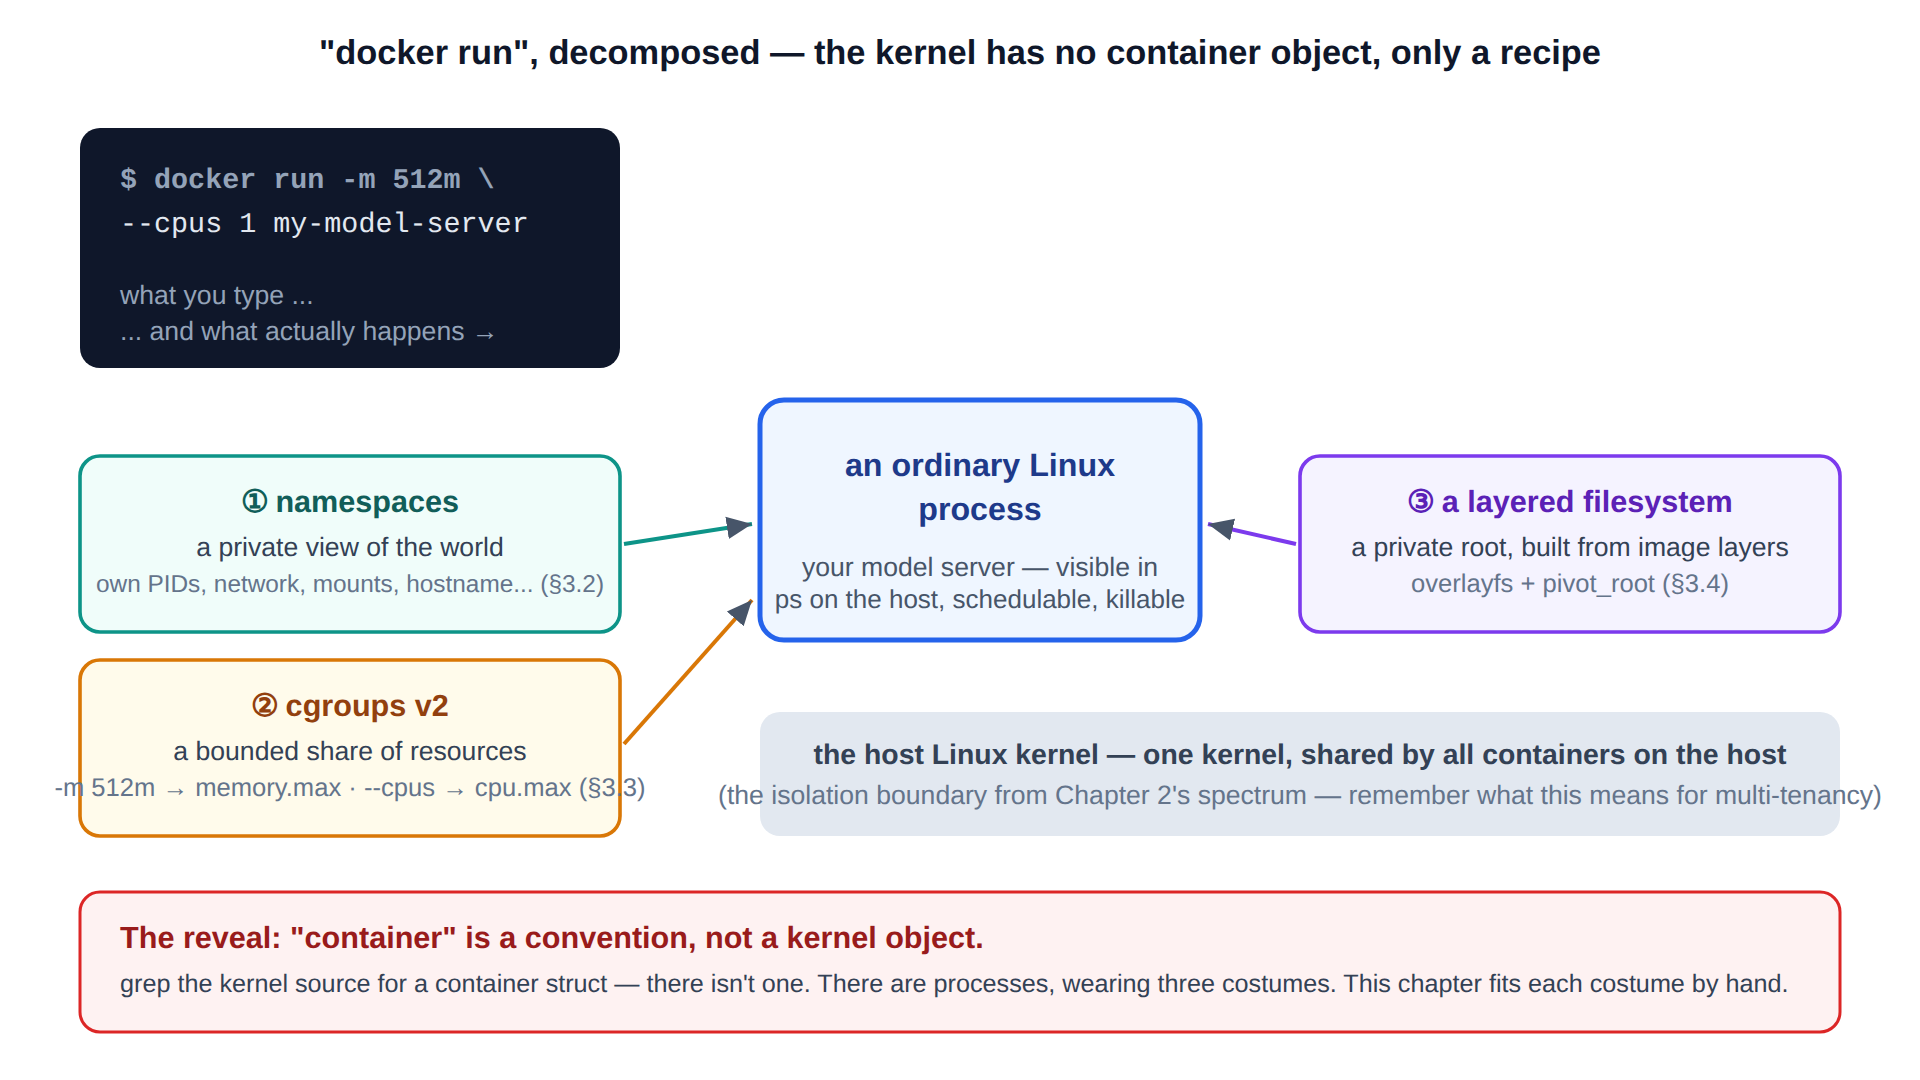
\includegraphics{figures/fig3-1_recipe.png}}\\[3pt]
  \figcaption{Figure 3-1  docker run, decomposed. The container is a recipe — namespaces + cgroups + a layered filesystem — applied to an ordinary process on a shared kernel.}
\end{tbbfigure}

\subsection*{Seeing it with your own eyes}

Claims like this should be checked, not believed. Start a container on any Docker-equipped machine, then interrogate it \textit{from the host} — not with Docker commands, but with the ordinary process tools you have used since your first OS course:

\begin{terminalbox}
\begin{Verbatim}[breaklines=true,breakanywhere=true,fontsize=\small,formatcom=\color{tbbtermfg},codes=\tbbcodeactive]
$ docker run -d --name demo -m 512m --cpus 1 python:3.11 sleep 9999
3f9a1c2b77e1...
$ docker inspect --format '{{.State.Pid}}' demo     # ask Docker for the host PID
41320
$ ps -o pid,ppid,rss,cmd -p 41320                  # plain ps, on the host
  PID   PPID   RSS  CMD
41320  41288  9184  sleep 9999
$ cat /proc/41320/cgroup                           # which budget group is it in?
0::/system.slice/docker-3f9a1c2b77e1....scope
$ cat /sys/fs/cgroup/system.slice/docker-3f9a*.scope/memory.max
536870912                                          # there is your -m 512m
$ ls -l /proc/41320/ns/pid                         # and its private view
... /proc/41320/ns/pid -> pid:[4026532871]
\end{Verbatim}
\end{terminalbox}
\figcaption{Transcript 3-1  A running container, interrogated from the host with ordinary process tools. It is a process (PID 41320) with a cgroup and namespaces attached.}

Read the transcript bottom-up and the whole chapter is previewed in five lines. The container is \textbf{visible in host ps} — it is process 41320, child of a runtime shim, using 9 MB of memory like any other process. Its \code{-m 512m} flag became \textbf{a number in a file} (\code{memory.max = 536870912} — Section 3.3). And its "isolation" is \textbf{a set of namespace links} under \code{/\allowbreak proc/\allowbreak 41320/\allowbreak ns/\allowbreak } (Section 3.2). The host kernel schedules this process, accounts for it, and — as Section 3.6 will show vividly — can kill it. Docker's contribution was orchestrating the setup, not conjuring a new kind of thing.

\subsection*{Why the demystification matters (and not just philosophically)}

Chapter 2's isolation spectrum already used this fact once: containers share the host kernel, which is why multi-tenant platforms reach for gVisor or microVMs. But the recipe view pays off operationally, every week of this course:

\begin{tbbitemize}
  \item \textbf{Your model server IS a container for the rest of this course.} Week 4 packages it as an image; Week 5 has Kubernetes schedule it; Weeks 9–12 serve from it. Everything those systems do to it — resource limits, health checks, networking, GPU access — bottoms out in this chapter's three mechanisms. When any of it misbehaves, the debugging happens at this layer.
  \item \textbf{The most common serving outage in the wild is this chapter's finale.} An inference pod that dies with \code{OOMKilled}, exit code 137, and no application log is not mysterious once you know that memory.max is a cgroup file and the OOM killer is its enforcement. Section 3.6 turns that from an incident into a checklist — with the actual \code{dmesg} lines and \code{kubectl} output you will someday read at 2 a.m.
  \item \textbf{Image layers are a latency budget.} A PyTorch/CUDA image weighs 5–10 GB; pulling it onto a fresh node is often the single largest line in Week 12's cold-start bill. Understanding overlayfs (3.4) — including why a \code{RUN rm} makes nothing smaller — is what makes image slimming rational rather than cargo-cult.
  \item \textbf{Debugging changes character.} When you know a container is a process, Transcript 3-1's toolbox works everywhere: \code{ps}, \code{/\allowbreak proc/\allowbreak <pid>/\allowbreak ns}, cgroup files, \code{nsenter} to step inside. The box stops being opaque, and "it works in the container" stops being the end of a conversation.
\end{tbbitemize}

The chapter's plan mirrors the recipe. Sections 3.2–3.4 take one ingredient each — seeing, using, being — each with transcripts and worked numbers. Section 3.5 assembles the ingredients into a working container with nothing but a shell, following the structure of Liz Rice's famous live-coding demo (this week's viewing). Sections 3.6–3.7 then spend the earned understanding on the single most valuable operational skill of the chapter: predicting, observing, and surviving the OOM killer.

\begin{calloutbox}{tbbpurple}{tbbpurplefill}
{\normalsize\bfseries\color{tbbpurple}Think About It}\par\vspace{3pt}
\begin{tbbitemize}
  \item Docker for Mac/Windows runs a Linux VM under the hood. Using this section's claim plus Chapter 2, explain why it must. What does that imply about "containers are lighter than VMs" on a laptop?
  \item In Transcript 3-1, sleep's parent is a "shim" process (PID 41288), not the docker CLI you typed into. Guess why a long-lived intermediary is useful (hint: what should happen to the container if the Docker daemon restarts?). Week 4 confirms.
  \item If a container is just a process, what does \code{docker exec} have to do? Sketch a guess (namespaces are the hint); check it against §3.2's setns.
\end{tbbitemize}
\end{calloutbox}

\section{Namespaces: A Private View of the World}

A namespace takes one global resource of the kernel — the process table, the network stack, the mount table — and gives a group of processes \textbf{their own private copy of the view}. Nothing is emulated and no second kernel appears (that was Chapter 2's move); the kernel simply keeps separate bookkeeping per namespace and shows each process the books it belongs to. When a process in a PID namespace calls \code{getpid()}, the kernel looks up which namespace the caller is in and returns the ID \textit{as seen from there}. Same kernel, same code path — different answer per viewer. Figure 3-2 tours the six classic namespaces through that lens: what the host sees versus what the container sees.

\begin{tbbfigure}
  \adjustbox{max width=0.94\linewidth,max totalheight=0.46\textheight}{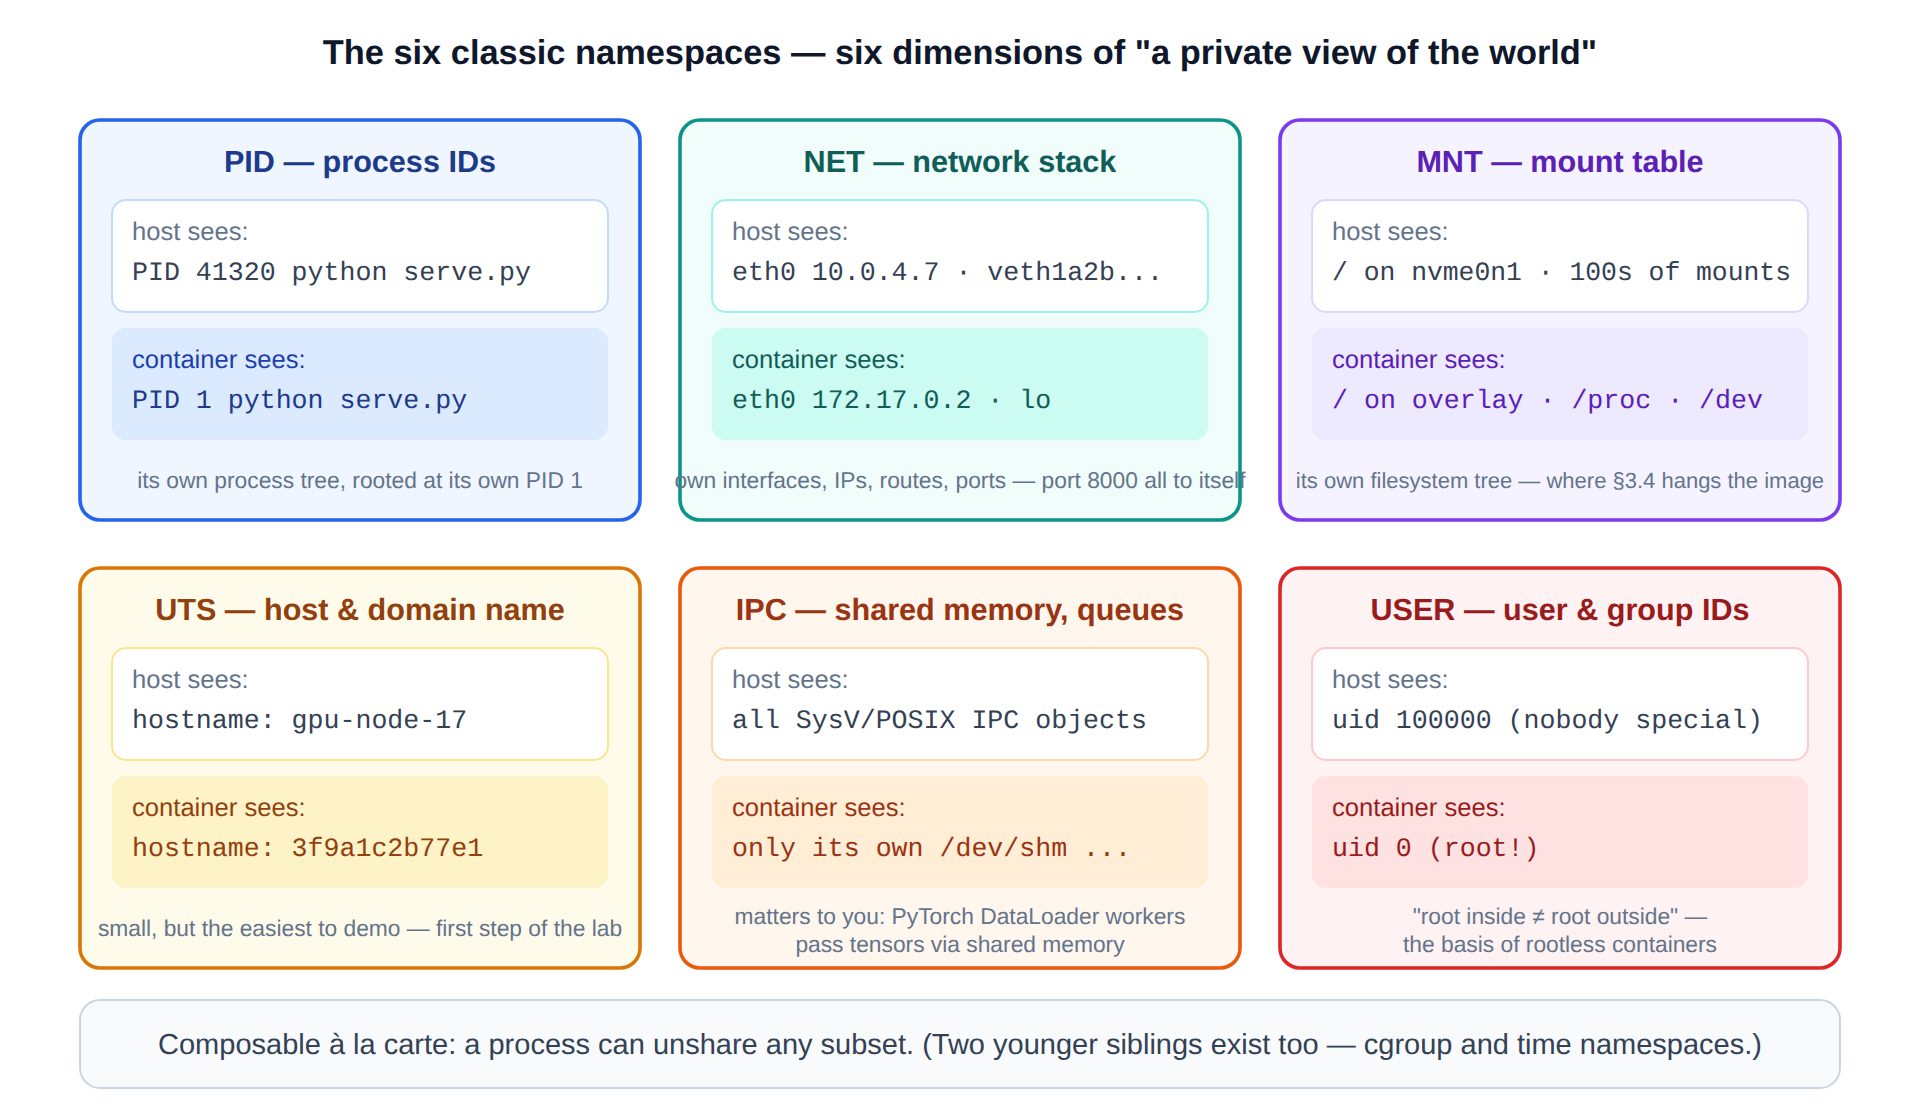
\includegraphics{figures/fig3-2_namespaces.png}}\\[3pt]
  \figcaption{Figure 3-2  Six namespaces, six dimensions of privacy: PIDs, network, mounts, hostname, IPC, and user IDs. Composable à la carte.}
\end{tbbfigure}

\subsection*{The API is three calls — and one directory}

For all its consequences, the namespace API is tiny. \code{unshare()} moves the \textit{calling} process into freshly created namespaces (the \code{unshare} command wraps it — the lab's workhorse). \code{clone()} creates a \textit{child} directly inside new namespaces — what container runtimes use. \code{setns()} \textit{joins} an existing namespace given a handle to it — and this one deserves a pause, because it answers Section 3.1's teaser: \code{docker exec} is \code{setns()} in a trench coat. It opens the target container's namespace files, joins them, and runs your shell there. No magic door; just a process changing which books it reads.

The handles live in a directory you can inspect. Every process exposes its namespace membership as symlinks in \code{/\allowbreak proc/\allowbreak <pid>/\allowbreak ns/\allowbreak }, and the bracketed number is the namespace's identity — \textbf{two processes are in the same namespace if and only if the numbers match}:

\begin{terminalbox}
\begin{Verbatim}[breaklines=true,breakanywhere=true,fontsize=\small,formatcom=\color{tbbtermfg},codes=\tbbcodeactive]
$ ls -l /proc/self/ns/            # my shell, on the host
mnt -> mnt:[4026531841]   net -> net:[4026531840]
pid -> pid:[4026531836]   uts -> uts:[4026531838]  ...
$ ls -l /proc/41320/ns/           # the container process from Transcript 3-1
mnt -> mnt:[4026532868]   net -> net:[4026532866]
pid -> pid:[4026532871]   uts -> uts:[4026532864]  ...
# every number differs -> different views on every axis.
# same number would mean: shared namespace. Free debugging test.
\end{Verbatim}
\end{terminalbox}
\figcaption{Transcript 3-2  Namespace identity is inspectable. Matching inode numbers = shared namespace — the first thing to check when "the container can't see X."}

Namespaces compose à la carte: a process can unshare only NET (common for network testing), or everything at once (a container). Two younger siblings — the cgroup namespace and the time namespace — round out the modern set of eight; the classic six carry this chapter.

\subsection*{PID: one process, two truths}

The PID namespace gives the container its own process tree, rooted at its own PID 1 (Figure 3-3, left). The same kernel task therefore has two identities — PID 41320 to the host, PID 1 to itself — and you can watch the second identity come into being:

\begin{terminalbox}
\begin{Verbatim}[breaklines=true,breakanywhere=true,fontsize=\small,formatcom=\color{tbbtermfg},codes=\tbbcodeactive]
$ sudo unshare --pid --fork --mount-proc bash    # new PID ns + fresh /proc
$ echo $$                                        # "what is my PID?"
1
$ ps aux
USER  PID  %CPU  %MEM  ... CMD
root    1   0.0   0.0  ... bash
root    8   0.0   0.0  ... ps aux
# two processes exist in this whole "machine" - and I am init.
\end{Verbatim}
\end{terminalbox}
\figcaption{Transcript 3-3  Inside a fresh PID namespace: the shell is PID 1 and the process table contains two entries. (--fork matters: PID membership applies to children, so unshare must fork the shell into the new world.)}

Why does the flag \code{--mount-proc} tag along? Because \code{ps} does not ask the kernel directly — it \textit{reads the /proc filesystem}, and if \code{/\allowbreak proc} still shows the host's mount, \code{ps} will happily report the host's thousands of processes even from inside the new namespace. Remounting \code{/\allowbreak proc} makes the tools tell the new truth. Keep this oddly philosophical lesson: \textbf{your view of a Linux system is only as honest as your mounts} — it returns in the lab (move 4) and as a monitoring footnote in Week 14.

\subsection*{Being PID 1 is a job, not just a number}

Unix assigns PID 1 (init) two duties that most application code has never had to think about — until it gets containerized and suddenly \textit{is} PID 1. First, \textbf{signals}: for PID 1, the kernel disables the default handlers that normally make SIGTERM fatal. A process with no explicit SIGTERM handler, running as PID 1, simply \textit{ignores} SIGTERM. Second, \textbf{reaping}: when a process dies, its parent must \code{wait()} on it to collect the exit status; until then it lingers as a \textbf{zombie} — a dead entry in the process table. Orphaned processes get re-parented to PID 1, so PID 1 must keep reaping other people's children forever, or zombies accumulate until \code{pids.max} (or the node) chokes.

Now play the tape of a Kubernetes rolling deploy (Week 13) against a model server that ignores both duties. At t=0, kubelet sends SIGTERM to PID 1 of the container — your Python server, which installed no handler. Nothing happens; the server keeps taking requests it will never finish. At t=30 s (the default grace period), kubelet loses patience and sends SIGKILL. The server dies mid-request; every in-flight request errors out; and this repeats \textbf{on every single deploy} — a permanent, self-inflicted outage generator that looks like "K8s being flaky." The fixes are small and standard:

\begin{tbbitemize}
  \item \textbf{Handle SIGTERM in the server}: stop accepting new requests, drain in-flight ones, then exit. (FastAPI/uvicorn and most serious servers do this if they receive the signal — see the next point.)
  \item \textbf{Make sure the signal reaches the server.} A classic Dockerfile bug: \code{CMD python serve.py} in \textit{shell form} runs \code{/\allowbreak bin/\allowbreak sh -c "python serve.py"} — the shell is PID 1, and it does not forward SIGTERM to its child. Use exec form (\code{CMD ["python", "serve.py"]}) so your server \textit{is} PID 1 and actually receives the signal.
  \item \textbf{Or install a real init}: \code{tini} (one flag: \code{docker run --init}) is a few-hundred-line PID 1 that forwards signals and reaps zombies, letting your application be an ordinary child again.
\end{tbbitemize}

\begin{tbbfigure}
  \adjustbox{max width=0.94\linewidth,max totalheight=0.46\textheight}{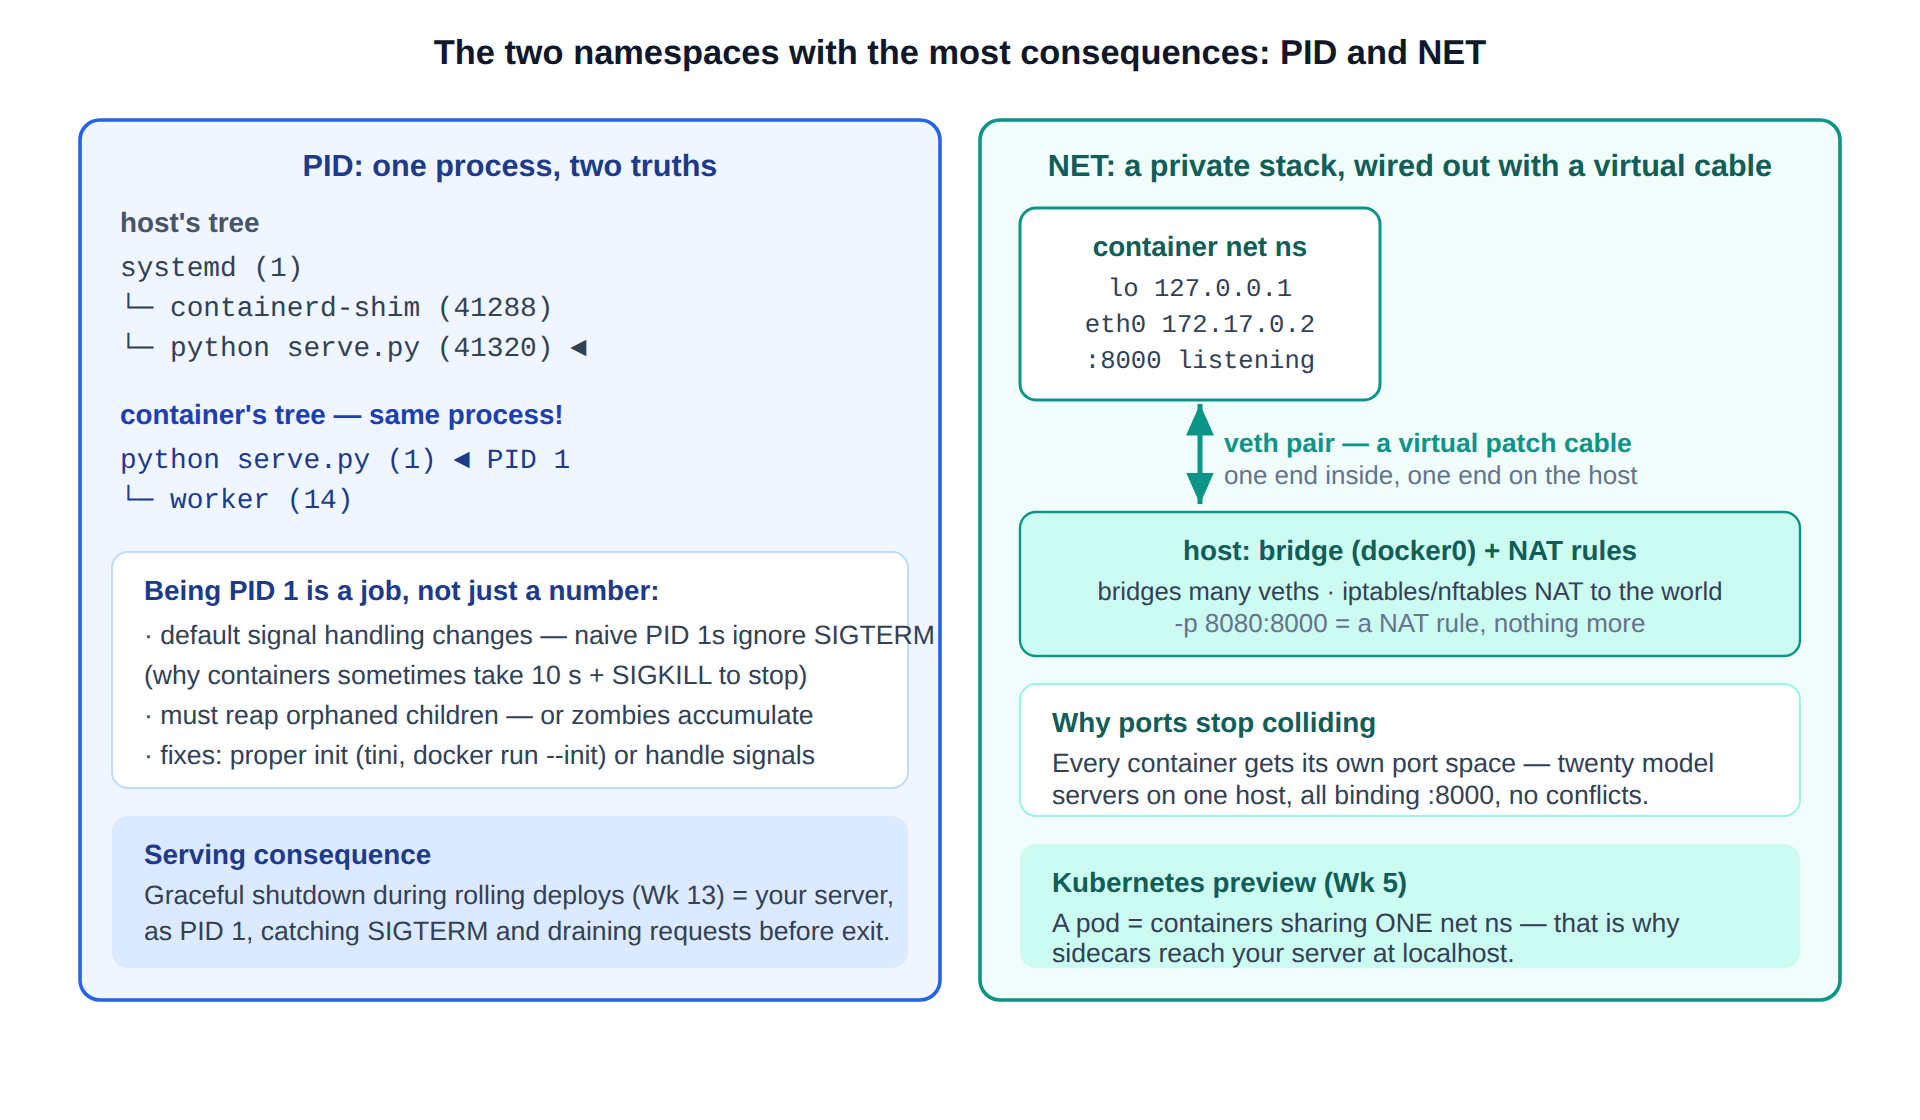
\includegraphics{figures/fig3-3_pidnet.png}}\\[3pt]
  \figcaption{Figure 3-3  The two consequential namespaces. Left: PID — one process, two identities, and PID 1's duties. Right: NET — a private stack wired out through a veth pair to a host bridge.}
\end{tbbfigure}

\subsection*{NET: a private stack, and the life of one request}

The NET namespace is the most physical-feeling of the six: the container gets an entire private network stack — interfaces, IP addresses, routing tables, firewall rules, and, crucially, \textbf{its own port space}. Twenty model-server replicas on one host can all bind \code{:8000} without a single conflict, which is what makes replica fleets administratively possible at all (nobody hands out port assignments like it's 1998).

A freshly private stack is also a freshly \textit{disconnected} one — a brand-new NET namespace contains only a loopback device, and even that is down. The standard wiring (Figure 3-3, right) creates a \textbf{veth pair} — two virtual NICs joined like a patch cable, Chapter 2's virtio spirit applied to networking — placing one end inside the container (renamed \code{eth0}) and the other on the host, plugged into a software \textbf{bridge} (Docker's \code{docker0}). To make it concrete, trace one request from your laptop to a container serving on port 8000, published with \code{-p 8080:8000}:

\begin{tbbitemize}
  \item \textbf{Arrive:} the packet hits the host's real NIC addressed to \code{host:8080}.
  \item \textbf{Translate:} an iptables/nftables DNAT rule — installed by Docker when you said \code{-p 8080:8000} — rewrites the destination to \code{172.17.0.2:8000}. \textit{A published port is literally one NAT rule.}
  \item \textbf{Bridge and cross:} the host routes the packet onto \code{docker0}, which forwards it down the container's veth; it emerges inside the NET namespace at \code{eth0}, where the server is listening on \code{:8000}.
  \item \textbf{Return:} the response retraces the path; connection tracking un-NATs the source so your laptop sees \code{host:8080} reply, none the wiser.
\end{tbbitemize}

One preview to file for Week 5: a Kubernetes \textbf{pod} is defined as containers sharing \textbf{one NET namespace} (via a tiny "pause" placeholder process that owns it). That single design decision is why sidecar proxies reach your model server at \code{localhost}, why "one IP per pod" is possible, and why two containers in a pod \textit{can} collide on ports while two pods never do.

\subsection*{USER: root inside is not root outside}

The USER namespace re-maps user IDs through an explicit table, \code{/\allowbreak proc/\allowbreak <pid>/\allowbreak uid\_map}. A mapping that reads \code{0 100000 65536} means: "uid 0 inside this namespace corresponds to uid 100000 outside, for a range of 65536 IDs." A process can thus \textit{be root inside} — install packages into its private filesystem, bind its private port 80 — while being unprivileged uid 100000 to the host kernel: touch a file inside and, from the host, it is owned by 100000, nobody special. This is the basis of \textbf{rootless containers} (Podman's trademark, Docker's rootless mode), where even the runtime runs unprivileged, and it takes a large bite out of container-escape consequences: an attacker who breaks out of a rootless container lands on the host as a nobody. (It is a mitigation, not the microVM boundary of Chapter 2 — the shared kernel's syscall surface remains.)

\subsection*{UTS and IPC, briefly — but not dismissively}

UTS (own hostname) is the smallest namespace and the best teacher: changing the hostname inside while watching the host stay unchanged is the fastest possible proof that views have really diverged, which is exactly why it is step 2 of the lab. IPC privatizes System V and POSIX shared memory — which sounds like an archaeology footnote until you remember that \textbf{PyTorch DataLoader workers pass tensors between processes through shared memory} mounted at \code{/\allowbreak dev/\allowbreak shm}. Docker defaults \code{/\allowbreak dev/\allowbreak shm} to 64 MB; the first time a multi-worker DataLoader moves real batches, it hits that ceiling and dies with a notoriously unhelpful \code{ERROR: Unexpected bus error encountered in worker. This might be caused by insufficient shared memory (shm)}. The fix every ML engineer eventually memorizes: \code{--shm-size=8g} (or K8s's equivalent volume). You now know which namespace that flag is talking to.

\begin{calloutbox}{tbbpurple}{tbbpurplefill}
{\normalsize\bfseries\color{tbbpurple}Think About It}\par\vspace{3pt}
\begin{tbbitemize}
  \item Two containers in one Kubernetes pod: using Figure 3-2's six axes, which namespaces do they share and which stay private? (You know enough to reason it out: they talk over localhost but have different filesystems.)
  \item Your server handles SIGTERM beautifully in local testing (python serve.py, Ctrl-C works) but ignores it in the container. Using this section, name the two most likely culprits and the one-line fix for each.
  \item Why is running as uid 0 inside a USER namespace much safer than uid 0 without one — yet still not as strong as Chapter 2's microVM boundary? Name the residual shared surface.
\end{tbbitemize}
\end{calloutbox}

\section{cgroups v2: A Bounded Share of the Machine}

Namespaces changed what a process can see; they place no limit on what it can consume. A containerized model server with a beautifully private PID tree can still eat every core and every byte of RAM on the node — and take nineteen neighbor replicas down with it. The second ingredient — \textbf{control groups, cgroups v2} — is the budget system: processes are placed into groups, and per-group \textbf{controllers} meter and limit CPU, memory, I/O, and process counts. Where namespaces answer "what world do I see?", cgroups answer "how much of the machine am I allowed?" (Figure 3-4).

\begin{tbbfigure}
  \adjustbox{max width=0.94\linewidth,max totalheight=0.46\textheight}{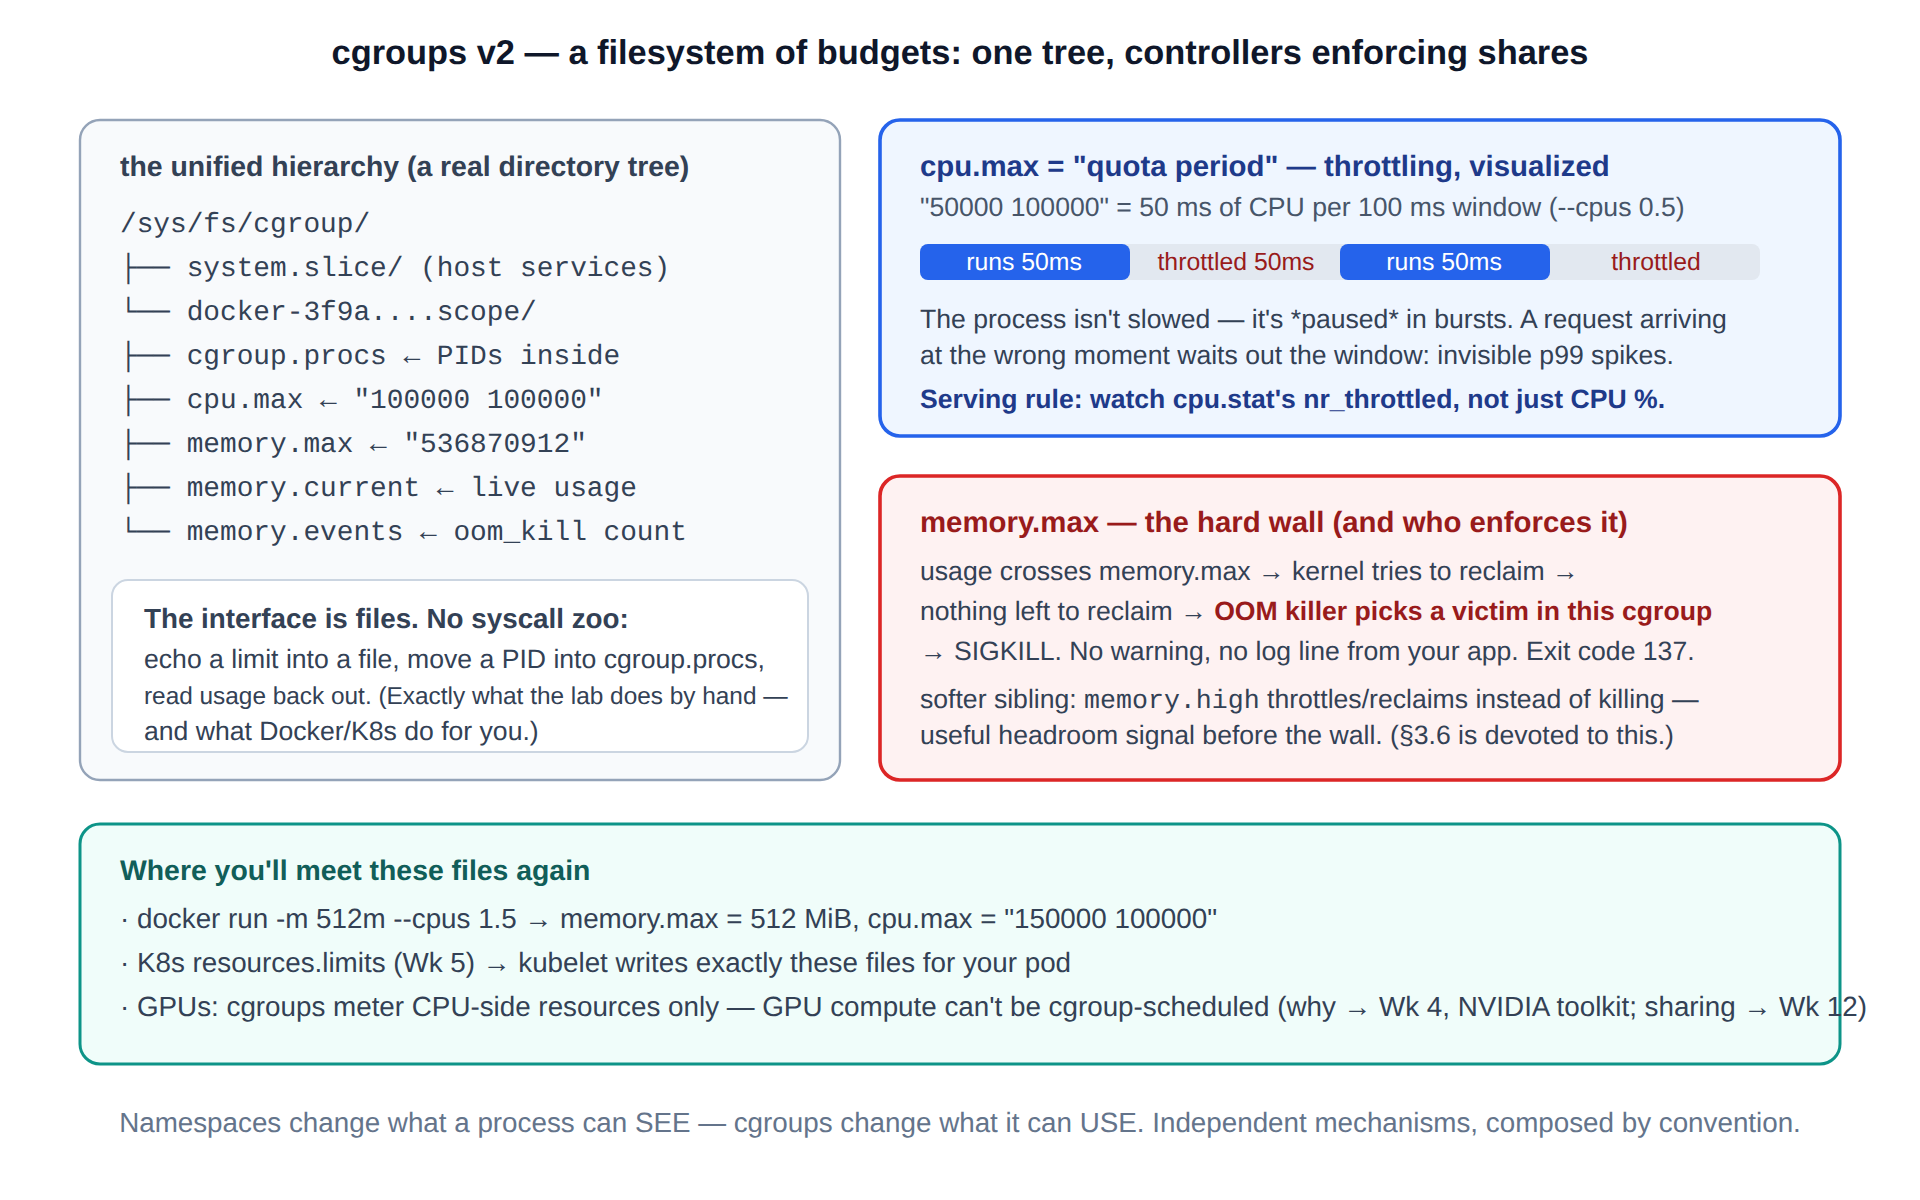
\includegraphics{figures/fig3-4_cgroups.png}}\\[3pt]
  \figcaption{Figure 3-4  cgroups v2: a single hierarchy exposed as a filesystem. cpu.max throttles in bursts (a p99 hazard); memory.max is a hard wall enforced by the OOM killer.}
\end{tbbfigure}

\subsection*{The interface is a filesystem — no library required}

cgroups v2 presents one unified tree under \code{/\allowbreak sys/\allowbreak fs/\allowbreak cgroup}, and the entire API is file operations. Watch a complete budget get built, applied, and read back — this is also a preview of the lab's move 5:

\begin{terminalbox}
\begin{Verbatim}[breaklines=true,breakanywhere=true,fontsize=\small,formatcom=\color{tbbtermfg},codes=\tbbcodeactive]
$ cd /sys/fs/cgroup && sudo mkdir demo        # a new group = a new directory
$ echo "50000 100000" | sudo tee demo/cpu.max # 50ms CPU per 100ms window (0.5 CPU)
$ echo $((256*1024*1024)) | sudo tee demo/memory.max   # 256 MiB hard wall
$ echo $$ | sudo tee demo/cgroup.procs        # enroll THIS shell (children follow)
$ cat demo/memory.current                     # live usage, in bytes
3862528
$ cat demo/cpu.stat | head -4
usage_usec 184220
user_usec  132009
system_usec 52211
nr_throttled 0                                # (watch this one in a moment)
\end{Verbatim}
\end{terminalbox}
\figcaption{Transcript 3-4  A complete cgroup budget in five file operations: mkdir, two echoes for limits, one echo to enroll, cat to observe. Docker and kubelet do exactly this on your behalf.}

That is the entire mechanism — \code{mkdir}, \code{echo}, \code{cat}. Recognize the ghostwriters (Table 3-2 below): a Docker flag or a Kubernetes limit is, in the end, a program writing numbers into these files. v2's single tree replaced v1's tangle of per-controller hierarchies; modern distributions and Kubernetes default to v2, and this course speaks v2 throughout.

\begin{tbbtablewrap}
  \begin{tabular}{@{}>{\raggedright\arraybackslash}m{\dimexpr 0.2447\tbltextwidth-2\tabcolsep\relax} >{\raggedright\arraybackslash}m{\dimexpr 0.4574\tbltextwidth-2\tabcolsep\relax} >{\raggedright\arraybackslash}m{\dimexpr 0.2979\tbltextwidth-2\tabcolsep\relax}@{}}
  \arrayrulecolor{tbbnavy}\specialrule{1pt}{0pt}{0pt}
  \rowcolor{tbbtablehead}{\centering \bfseries\color{tbbnavy}File} & {\centering \bfseries\color{tbbnavy}Meaning} & {\centering \bfseries\color{tbbnavy}Typical writer} \\
  \arrayrulecolor{tbbnavy}\specialrule{0.7pt}{0pt}{2pt}
  {\textbf{cgroup.procs}} & {PIDs enrolled in this group (write to move a process in)} & {runtime / you (lab)} \\
  \arrayrulecolor{tbbtableborder}\hline
  {\textbf{cpu.max}} & {Hard quota: "<quota> <period>" in µs, e.g. "50000 100000" = 0.5 CPU} & {docker --cpus, kubelet (limits)} \\
  \arrayrulecolor{tbbtableborder}\hline
  {\textbf{cpu.weight}} & {Proportional share (1–10000) under contention; soft, work-conserving} & {kubelet (from requests)} \\
  \arrayrulecolor{tbbtableborder}\hline
  {\textbf{cpu.stat}} & {Usage + nr\_throttled / throttled\_usec — the throttling diagnostic} & {(read-only telemetry)} \\
  \arrayrulecolor{tbbtableborder}\hline
  {\textbf{memory.max}} & {Hard memory wall; crossing it after failed reclaim → OOM kill} & {docker -m, kubelet (limits)} \\
  \arrayrulecolor{tbbtableborder}\hline
  {\textbf{memory.high}} & {Soft ceiling: throttle + reclaim, no kill — the tripwire (§3.6)} & {you / platform policy} \\
  \arrayrulecolor{tbbtableborder}\hline
  {\textbf{memory.current}} & {Live usage of the group — what you watch in the lab} & {(read-only telemetry)} \\
  \arrayrulecolor{tbbtableborder}\hline
  {\textbf{memory.events}} & {Counters incl. oom\_kill — the OOM evidence ledger} & {(read-only telemetry)} \\
  \arrayrulecolor{tbbtableborder}\hline
  {\textbf{pids.max}} & {Max processes/threads — the fork-bomb fence} & {docker --pids-limit} \\
  \arrayrulecolor{tbbnavy}\specialrule{1pt}{2pt}{0pt}
  \end{tabular}\par
  \figcaption{Table 3-1  The cgroup v2 files you will actually touch}
\end{tbbtablewrap}

\subsection*{CPU: quotas throttle in bursts — a worked latency example}

The CPU controller has two knobs with \textit{very} different personalities. \code{cpu.weight} divides CPU proportionally \textbf{under contention only}: weights 300 vs. 100 on a busy 4-core box yield roughly 3 cores vs. 1 — but if the neighbor goes idle, either group may use everything. It is \textit{work-conserving}: no cycles are ever wasted to enforce it. \code{cpu.max} is a hard quota with a period: \code{"50000 100000"} means \textit{this group may run 50 ms out of every 100 ms window}, idle neighbors or not. And the enforcement style is the crucial subtlety: not a smooth 2× slowdown, but \textbf{throttling} — the group runs at full native speed until its quota for the window is spent, then is frozen until the next window opens.

Feel it with arithmetic. Suppose an inference request needs \textbf{30 ms of CPU time}, and the container's quota is \code{"20000 100000"} (0.2 CPU — a value real clusters set on "small" services). Best case, the request arrives at the start of a fresh window: it runs 20 ms, hits the quota, \textbf{freezes for 80 ms}, runs its last 10 ms in the next window — completing after \textbf{110 ms}, of which 80 ms was enforced pause. Worst case, it arrives just after the quota was spent by earlier requests: add up to another 80 ms of waiting before it runs at all — approaching \textbf{190 ms} for 30 ms of work. Meanwhile a lightly loaded p50 request may fit entirely inside a window and see none of this. That is the signature: \textbf{p50 fine, p99 spiky in \textasciitilde{}multiples of the window remainder, application profiler blind} — the process was not running, so there is nothing to profile.

\begin{terminalbox}
\begin{Verbatim}[breaklines=true,breakanywhere=true,fontsize=\small,formatcom=\color{tbbtermfg},codes=\tbbcodeactive]
# after driving load through the throttled cgroup from Transcript 3-4:
$ cat demo/cpu.stat
usage_usec     9184220
nr_periods     412
nr_throttled   118        # windows in which we hit the quota
throttled_usec 8221340    # 8.2 s of enforced pause, total
\end{Verbatim}
\end{terminalbox}
\figcaption{Transcript 3-5  The throttling diagnostic. nr\_throttled climbing under load = your p99 spikes are manufactured here, not in your code.}

The standard remedies follow from the mechanism: raise the quota; prefer \textbf{weights} (requests) over hard caps for latency-critical pods so idle capacity stays usable; or shorten the effective pause by understanding what your platform sets (Week 5 returns to the "should K8s CPU limits even be set?" debate with this section as ammunition). File the whole story next to Chapter 2's steal time: \textbf{two different mechanisms, one lesson — tail latency can be manufactured a layer below your code.}

\subsection*{Memory: a hard wall with an enforcer — and a reclaim subtlety}

The memory controller's \code{memory.max} is a genuinely hard limit, but the path to the wall has a stop the naive picture misses: \textbf{reclaim}. When a group's usage reaches the limit, the kernel first tries to free memory it can recreate — above all \textbf{page cache} (file contents cached in RAM). This matters for reading dashboards: \code{memory.current} counts page cache, so a container that streams large files (say, loading model weights) can \textit{look} pinned at its limit for hours while being perfectly healthy — the cache is reclaimable ballast, not need. What cannot be reclaimed is \textbf{anonymous memory}: your Python heap, your tensors. When usage at the wall is anonymous, reclaim fails — and the kernel invokes the \textbf{OOM killer scoped to this cgroup}, which picks the group's biggest process (tunable via \code{oom\_score\_adj}) and delivers SIGKILL: unappealable, uncatchable, invisible to the victim. The application logs nothing; the shell sees \textbf{exit code 137} (128 + 9); Kubernetes stamps \code{OOMKilled}. Its gentler sibling \code{memory.high} throttles and aggressively reclaims \textit{without} killing — the tripwire you will learn to set in Section 3.6, which owns the full story from here.

\subsection*{What cgroups can and cannot referee}

Rounding out the controllers: \code{io} meters block-device bandwidth and IOPS (relevant when weight-loading hammers a shared disk), \code{pids} caps process counts (the fork-bomb fence from Liz Rice's demo), and \code{cpuset} pins groups to specific cores (the container cousin of Chapter 2's dedicated-core instances). Note also the negative space, because it shapes this course: \textbf{cgroups have no GPU controller.} The kernel can gate \textit{access} to \code{/\allowbreak dev/\allowbreak nvidia*} devices — that is how \code{--gpus} works at the permission level (Week 4 shows the toolkit plumbing) — but nothing in the cgroup tree can slice GPU compute time or partition VRAM the way \code{cpu.max} and \code{memory.max} slice their resources. Concretely: put two processes on one GPU and nothing stops either from \code{cudaMalloc}-ing all of VRAM or monopolizing the SMs. That absence is precisely why GPU sharing needed the vendor mechanisms of Chapter 2 — time-slicing, MPS, MIG — and why Week 12's GPU-sharing toolbox looks nothing like this section.

\begin{tbbtablewrap}
  \begin{tabular}{@{}>{\raggedright\arraybackslash}m{\dimexpr 0.3511\tbltextwidth-2\tabcolsep\relax} >{\raggedright\arraybackslash}m{\dimexpr 0.3298\tbltextwidth-2\tabcolsep\relax} >{\raggedright\arraybackslash}m{\dimexpr 0.3191\tbltextwidth-2\tabcolsep\relax}@{}}
  \arrayrulecolor{tbbnavy}\specialrule{1pt}{0pt}{0pt}
  \rowcolor{tbbtablehead}{\centering \bfseries\color{tbbnavy}What you write} & {\centering \bfseries\color{tbbnavy}What lands in cgroup v2} & {\centering \bfseries\color{tbbnavy}Notes} \\
  \arrayrulecolor{tbbnavy}\specialrule{0.7pt}{0pt}{2pt}
  {docker run -m 512m} & {memory.max = 536870912} & {hard wall; §3.6's subject} \\
  \arrayrulecolor{tbbtableborder}\hline
  {docker run --cpus 1.5} & {cpu.max = "150000 100000"} & {burst-throttled, not smoothed} \\
  \arrayrulecolor{tbbtableborder}\hline
  {docker run --pids-limit 256} & {pids.max = 256} & {fork-bomb fence} \\
  \arrayrulecolor{tbbtableborder}\hline
  {K8s resources.requests (Wk 5)} & {cpu.weight (+ scheduler math)} & {planning + soft shares} \\
  \arrayrulecolor{tbbtableborder}\hline
  {K8s resources.limits (Wk 5)} & {cpu.max, memory.max} & {exactly this section's walls} \\
  \arrayrulecolor{tbbtableborder}\hline
  {docker run --gpus all (Wk 4)} & {— no cgroup controller —} & {device access only; sharing needs Ch. 2's vGPU/MIG (Wk 12)} \\
  \arrayrulecolor{tbbnavy}\specialrule{1pt}{2pt}{0pt}
  \end{tabular}\par
  \figcaption{Table 3-2  How the tools you use ghostwrite these files}
\end{tbbtablewrap}

\begin{calloutbox}{tbbpurple}{tbbpurplefill}
{\normalsize\bfseries\color{tbbpurple}Think About It}\par\vspace{3pt}
\begin{tbbitemize}
  \item A latency-sensitive inference pod is set to cpu.max = "100000 100000" (1 CPU). Under load, p50 is fine but p99 shows 40–90 ms spikes and nr\_throttled is climbing. Using the worked example's arithmetic, explain the spike sizes and propose two distinct fixes with their trade-offs.
  \item Your dashboard shows a weight-loading container pinned at 98\% of memory.max for an hour, yet no OOM kill occurs. Using the reclaim subtlety, explain why — and name the file that would tell you how close to real danger it is.
  \item Why is "memory limit = observed idle memory + 10\%" a recipe for OOM kills for an inference server, when the same rule works fine for many stateless web apps? (You can answer from Chapter 1; §3.6 will confirm with numbers.)
\end{tbbitemize}
\end{calloutbox}

\section{overlayfs: The Filesystem Is Layers}

The third ingredient answers "where does the container's world come from?" A container needs a private root filesystem — its own \code{/\allowbreak usr/\allowbreak bin/\allowbreak python}, its own libraries — that (a) can be shipped around as an artifact, (b) doesn't cost a full copy per container, and (c) appears in milliseconds. The mechanism behind all three is \textbf{overlayfs}, a union filesystem that \textit{stacks} directories: several read-only \textbf{lower} directories (the image layers), one writable \textbf{upper} directory (the container's scratch space), presented as a single \textbf{merged} view that the container mounts as \code{/\allowbreak } (Figure 3-5).

\begin{tbbfigure}
  \adjustbox{max width=0.94\linewidth,max totalheight=0.46\textheight}{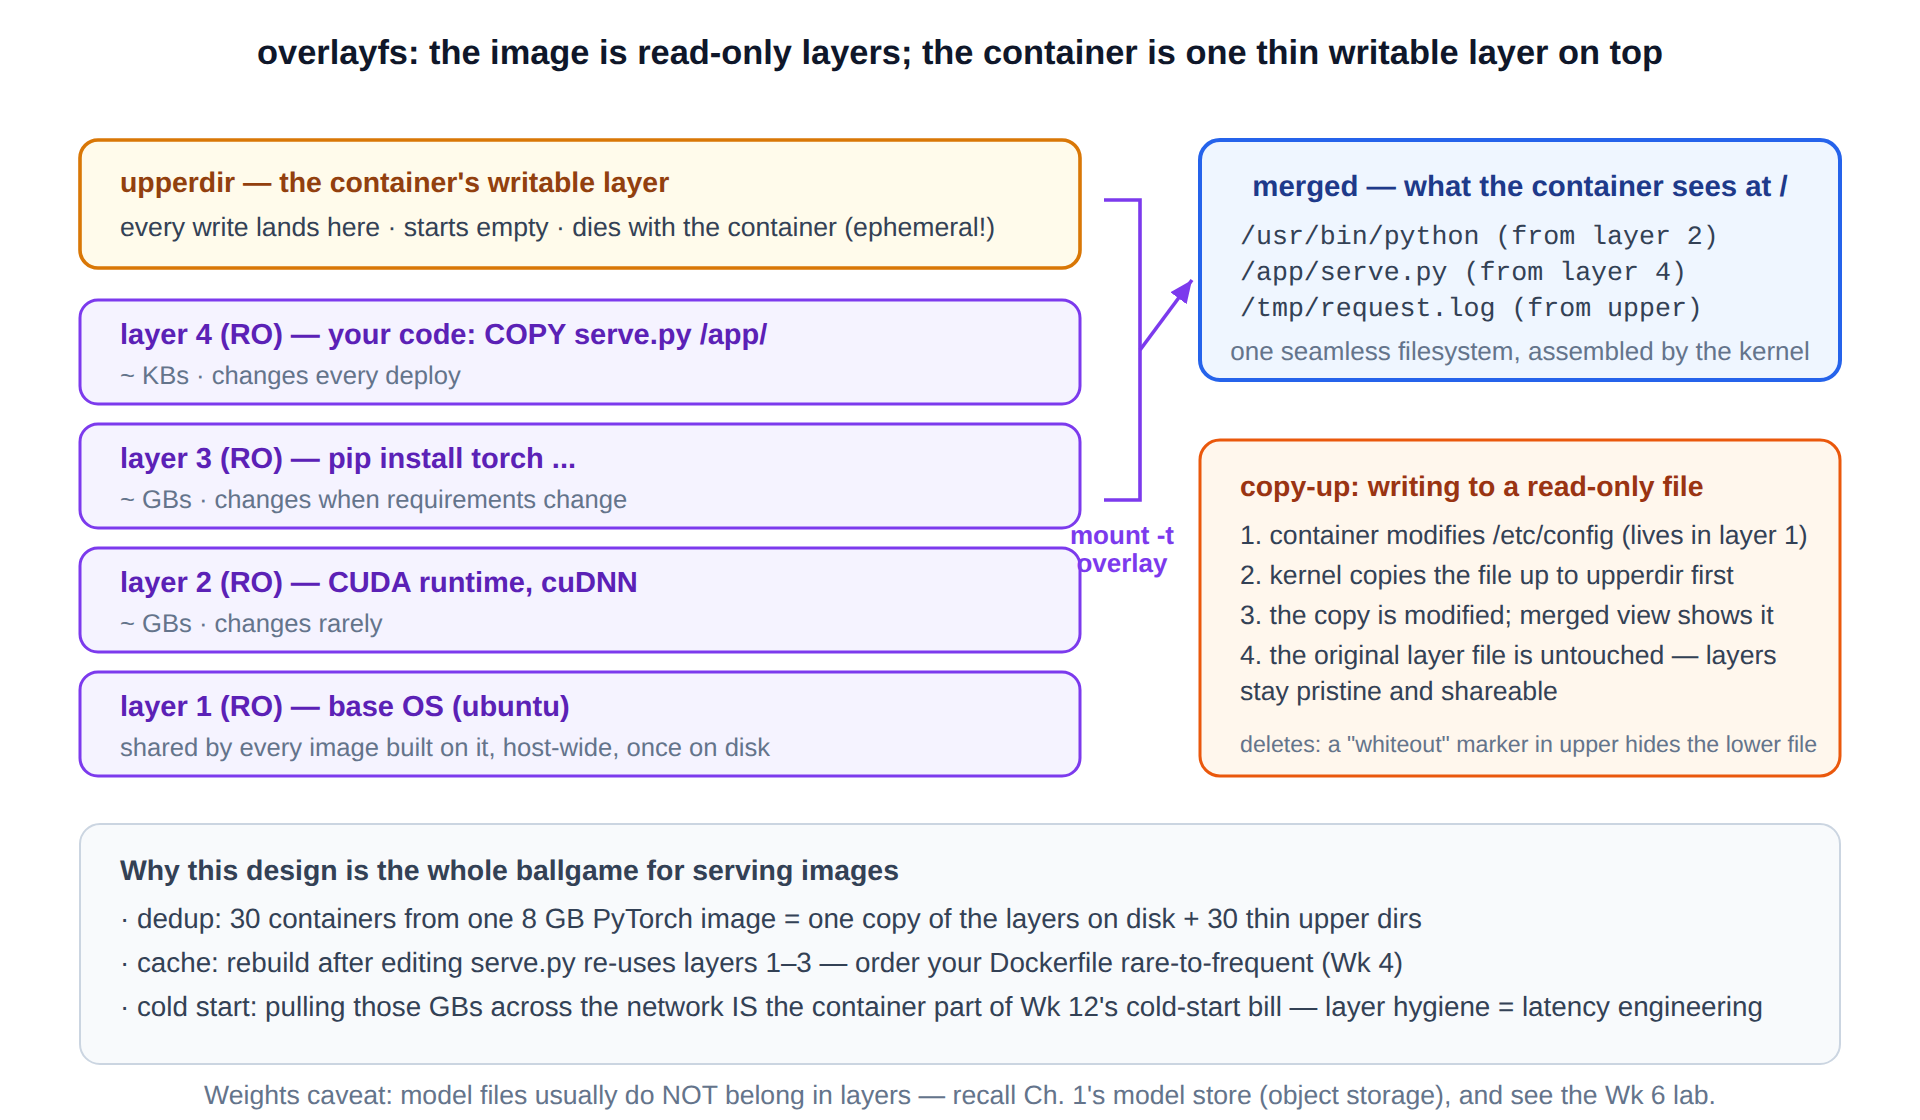
\includegraphics{figures/fig3-5_overlayfs.png}}\\[3pt]
  \figcaption{Figure 3-5  overlayfs: read-only image layers + one thin writable layer = the container's root. Writes copy-up; deletes leave whiteouts; layers stay pristine and shared.}
\end{tbbfigure}

\subsection*{The three rules, demonstrated in ninety seconds}

overlayfs is a mount type in every stock Linux kernel — you can play the whole game in a scratch directory, no Docker involved. The transcript below is worth actually running; each command teaches one of the three rules:

\begin{terminalbox}
\begin{Verbatim}[breaklines=true,breakanywhere=true,fontsize=\small,formatcom=\color{tbbtermfg},codes=\tbbcodeactive]
$ mkdir lower upper work merged
$ echo "from the image"  > lower/config.txt
$ echo "also the image"  > lower/keep.txt
$ sudo mount -t overlay overlay \
    -o lowerdir=lower,upperdir=upper,workdir=work merged
$ cat merged/config.txt                # RULE 1 - reads fall through
from the image
$ echo "changed!" > merged/config.txt  # RULE 2 - writes copy-up
$ cat lower/config.txt                 #   the layer is untouched...
from the image
$ ls upper/                            #   ...the copy lives in upper
config.txt
$ rm merged/keep.txt                   # RULE 3 - deletes leave whiteouts
$ ls -l upper/keep.txt
c--------- 1 root root 0, 0 ... upper/keep.txt   # a marker, not a file
$ ls lower/                            #   the bytes still exist below!
config.txt  keep.txt
\end{Verbatim}
\end{terminalbox}
\figcaption{Transcript 3-6  overlayfs in one sitting: reads fall through the stack, writes copy the file up before touching it, deletes hide files with whiteout markers — lower layers stay pristine and shareable.}

Three rules, now with their consequences spelled out. \textbf{Reads search top-down}, so the merged view shows the uppermost version of each path — that is how a later layer "updates" a file without modifying the earlier layer. \textbf{Writes trigger copy-up}: the whole file is copied to the upper directory first, and the copy is what changes; every container gets its own upper, so thirty containers can "modify" the same base image while sharing every read-only byte of it. \textbf{Deletes leave whiteouts} — that character-device marker (\code{c---------}, device 0:0) hides \code{keep.txt} from the merged view while the bytes remain in the lower layer. The whiteout rule has a famous financial consequence: \textbf{a RUN rm in a later Dockerfile layer makes the image larger, not smaller} — the "deleted" bytes still ship in the earlier layer, plus a marker. Deleting must happen \textit{in the same layer that created the files}, which in Dockerfile terms means the same \code{RUN} line:

\begin{terminalbox}
\begin{Verbatim}[breaklines=true,breakanywhere=true,fontsize=\small,formatcom=\color{tbbtermfg},codes=\tbbcodeactive]
# WRONG - image contains 900MB of downloads AND a whiteout hiding them:
RUN apt-get install -y build-essential
RUN rm -rf /var/lib/apt/lists /tmp/downloads

# RIGHT - the layer never contains the junk at all:
RUN apt-get install -y build-essential && \
    rm -rf /var/lib/apt/lists /tmp/downloads
\end{Verbatim}
\end{terminalbox}
\figcaption{Transcript 3-7  The whiteout rule as Dockerfile practice: cleanup must share a RUN with the mess it cleans, or the bytes ship anyway.}

\subsection*{Why layers are an economic design — with your serving image as the ledger}

Now read the stack as an economist, using the image you will actually build in Week 4's lab. A serving image decomposes naturally by \textit{rate of change}, and a well-ordered Dockerfile puts the slowest-changing content lowest:

\begin{tbbtablewrap}
  \begin{tabular}{@{}>{\raggedright\arraybackslash}m{\dimexpr 0.3617\tbltextwidth-2\tabcolsep\relax} >{\raggedright\arraybackslash}m{\dimexpr 0.1809\tbltextwidth-2\tabcolsep\relax} >{\raggedright\arraybackslash}m{\dimexpr 0.2234\tbltextwidth-2\tabcolsep\relax} >{\raggedright\arraybackslash}m{\dimexpr 0.2340\tbltextwidth-2\tabcolsep\relax}@{}}
  \arrayrulecolor{tbbnavy}\specialrule{1pt}{0pt}{0pt}
  \rowcolor{tbbtablehead}{\centering \bfseries\color{tbbnavy}Layer (Dockerfile step)} & {\centering \bfseries\color{tbbnavy}Size (typ.)} & {\centering \bfseries\color{tbbnavy}Changes...} & {\centering \bfseries\color{tbbnavy}Rebuild/pull cost} \\
  \arrayrulecolor{tbbnavy}\specialrule{0.7pt}{0pt}{2pt}
  {FROM ubuntu / python-slim base} & {\textasciitilde{}80–150 MB} & {yearly} & {cached \textasciitilde{}forever} \\
  \arrayrulecolor{tbbtableborder}\hline
  {CUDA runtime + cuDNN libs} & {\textasciitilde{}2–3 GB} & {per CUDA upgrade} & {cached for months} \\
  \arrayrulecolor{tbbtableborder}\hline
  {pip install torch + deps} & {\textasciitilde{}2–3 GB} & {when requirements.txt changes} & {cached for weeks} \\
  \arrayrulecolor{tbbtableborder}\hline
  {\textbf{COPY serve.py /app/}} & {\textbf{\textasciitilde{}40 KB}} & {\textbf{every deploy}} & {\textbf{seconds}} \\
  \arrayrulecolor{tbbnavy}\specialrule{1pt}{2pt}{0pt}
  \end{tabular}\par
  \figcaption{Table 3-3  A model-server image, layer by layer (representative sizes)}
\end{tbbtablewrap}

This ordering buys three things this course keeps paying for. \textbf{Dedup:} thirty replicas of that \textasciitilde{}5–6 GB image on one node store the layers \textit{once} plus thirty near-empty upper dirs — this is why container density is even possible with ML images. \textbf{Cache:} editing \code{serve.py} and rebuilding reuses every layer below it — a seconds-long rebuild and a kilobytes-long push, versus the 20-minute, multi-gigabyte disaster you get if \code{COPY . /\allowbreak app} sits \textit{above} \code{pip install} (the classic beginner inversion: now every code edit invalidates the dependency layer and rebuilds torch). \textbf{Startup:} "starting" a container's filesystem is one overlay mount of already-present layers — milliseconds — so the filesystem is never the cold-start problem. \textit{Pulling absent layers over the network is.} Run the Week-12-preview arithmetic once: a 6 GB image onto a fresh node at an effective 100–250 MB/s (registry, network, and decompression all taxing the pipe) is \textbf{25–60 seconds of cold start before a single line of your code runs} — usually the largest single line item, and the reason layer hygiene is latency engineering, not tidiness.

One serving-specific caveat completes the picture: \textbf{model weights usually do not belong in image layers.} Weights are huge, change on a different cadence than code, and (Chapter 1) live properly in a model store on object storage, loaded at startup — the Week 6 lab builds exactly that path, and Week 13's registry/versioning story depends on it. Baking a 30 GB checkpoint into a layer couples model versioning to image versioning, bloats every node's disk, and makes each deploy re-ship unchanged gigabytes. It is occasionally the right call (immutable demo images, edge appliances); it should be a decision, not a default.

\begin{calloutbox}{tbbpurple}{tbbpurplefill}
{\normalsize\bfseries\color{tbbpurple}Think About It}\par\vspace{3pt}
\begin{tbbitemize}
  \item A teammate's Dockerfile: FROM python-slim → COPY . /app → pip install -r /app/requirements.txt → CMD .... Predict the rebuild behavior when (a) serve.py changes, (b) requirements.txt changes. Reorder it properly and state the new costs for each case.
  \item Using Transcript 3-6's rules: two containers from the same image both append to /var/log/app.log inside. Do they see each other's lines? Where do the two files physically live? What happens to both at container removal?
  \item Estimate: your team pushes 6 deploys/day of a 5.5 GB image where only serve.py (40 KB) changes. With proper layering, how many bytes move per deploy? With COPY-above-pip inversion? (Registry egress is billed — Ch. 1's cost lens applies.)
\end{tbbitemize}
\end{calloutbox}

\section{Build One by Hand — and What Docker Actually Adds}

Time to assemble the recipe with bare hands. The sequence below is the intellectual core of this week's lab and follows the shape of Liz Rice's celebrated "Containers from Scratch" demo (she live-codes it in Go; you will do it with stock shell commands, which is even more demystifying). Five moves, each cashing in one section of this chapter (Figure 3-6) — run them in order and read every output.

\begin{tbbfigure}
  \adjustbox{max width=0.94\linewidth,max totalheight=0.46\textheight}{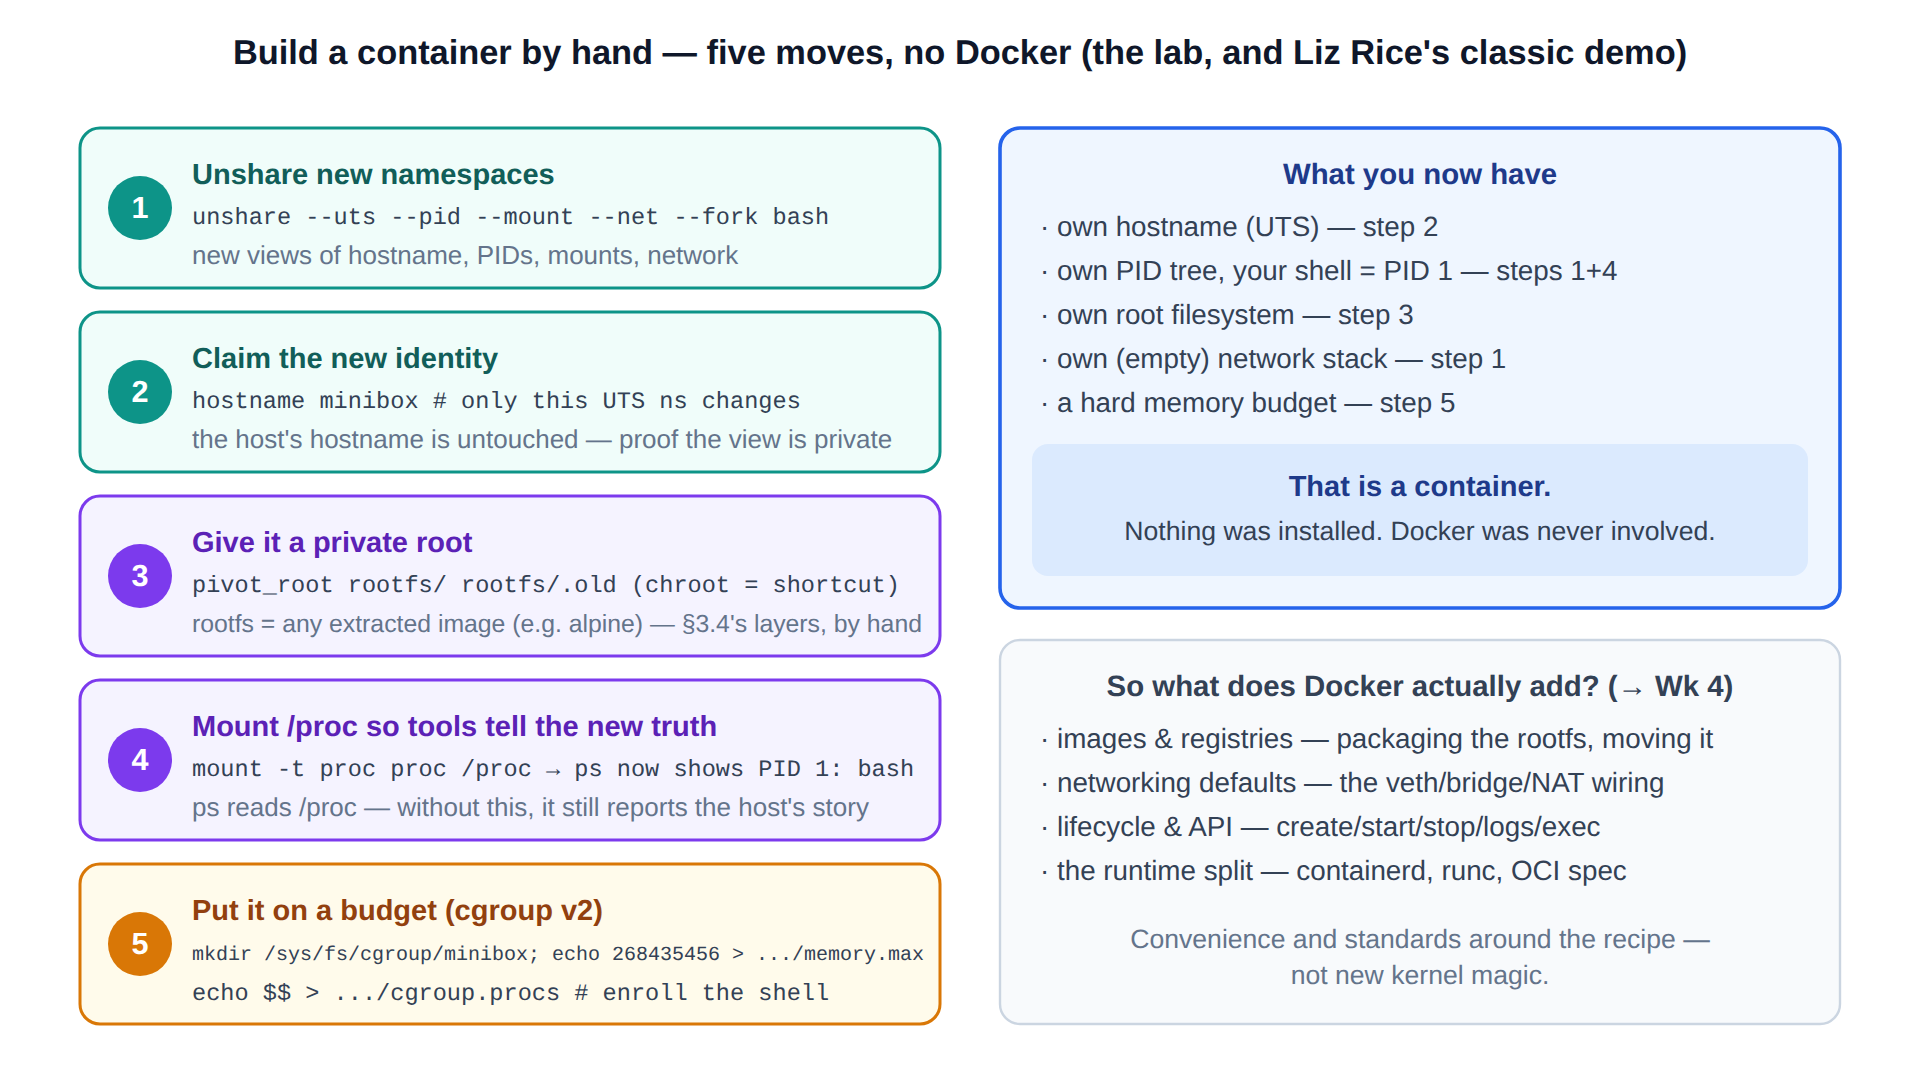
\includegraphics{figures/fig3-6_byhand.png}}\\[3pt]
  \figcaption{Figure 3-6  A container in five moves: unshare namespaces, claim an identity, pivot to a private root, mount /proc, enroll in a cgroup. Docker adds convenience and standards — not kernel magic.}
\end{tbbfigure}

\subsection*{Moves 1–2: new views, and proof they are private}

\begin{terminalbox}
\begin{Verbatim}[breaklines=true,breakanywhere=true,fontsize=\small,formatcom=\color{tbbtermfg},codes=\tbbcodeactive]
$ sudo unshare --uts --pid --mount --net --fork bash   # MOVE 1
# (prompt looks identical - but check your namespace links vs Transcript 3-2)
$ hostname minibox                                     # MOVE 2
$ hostname
minibox
# ...meanwhile, in a second terminal on the host:
$ hostname
gpu-node-17                    # untouched. The view really is private.
\end{Verbatim}
\end{terminalbox}
\figcaption{Transcript 3-8  Moves 1–2. The --fork matters (PID membership applies to children); the two-terminal hostname contrast is your first lab artifact.}

\subsection*{Move 3: a private root (and why pivot\_root, not chroot)}

Unpack any small rootfs — an alpine or ubuntu-base tarball, which is literally an image's layers flattened into one directory — and make it \code{/\allowbreak }. The demo shortcut is \code{chroot}, and for the lab it is fine. Real runtimes use \code{pivot\_root}, and the difference is worth one sentence of security literacy: \code{chroot} merely \textit{repoints} the process's idea of \code{/\allowbreak } while the old root remains in the mount namespace — reachable again via well-known escape tricks (a process holding a file descriptor outside the jail can walk back out) — whereas \code{pivot\_root} \textit{swaps} the mount namespace's root and lets you unmount the old world entirely. Repoint versus replace: the classic container-security footnote, now yours.

\begin{terminalbox}
\begin{Verbatim}[breaklines=true,breakanywhere=true,fontsize=\small,formatcom=\color{tbbtermfg},codes=\tbbcodeactive]
$ curl -LO https://.../alpine-minirootfs-3.20-x86_64.tar.gz   # ~3 MB(!)
$ mkdir rootfs && tar -xzf alpine-minirootfs-*.tar.gz -C rootfs
$ ls rootfs
bin  dev  etc  home  lib  ...  usr  var        # a whole tiny Linux userland
$ chroot rootfs /bin/sh                        # MOVE 3 (lab shortcut)
/ # ls /                                       # your / is now the rootfs
bin  dev  etc  home  lib  ...  usr  var
\end{Verbatim}
\end{terminalbox}
\figcaption{Transcript 3-9  Move 3. A rootfs is just a directory; an image is just a shipped rootfs (in layers). Alpine's is 3 MB — perspective for your 6 GB CUDA image.}

\subsection*{Move 4: make the tools tell the new truth}

\begin{terminalbox}
\begin{Verbatim}[breaklines=true,breakanywhere=true,fontsize=\small,formatcom=\color{tbbtermfg},codes=\tbbcodeactive]
/ # ps aux                       # BEFORE mounting /proc: confusion
ps: can't open /proc: No such file or directory
/ # mount -t proc proc /proc     # MOVE 4
/ # ps aux
PID   USER   COMMAND
  1   root   /bin/sh             # there it is: you are init
  9   root   ps aux
\end{Verbatim}
\end{terminalbox}
\figcaption{Transcript 3-10  Move 4. ps reads /proc; mount the namespace-aware proc and the tools report the new world — two processes, and your shell is PID 1.}

\subsection*{Move 5: a budget — and the complete inventory}

From the host (second terminal), build the cgroup exactly as in Transcript 3-4 — \code{mkdir /\allowbreak sys/\allowbreak fs/\allowbreak cgroup/\allowbreak minibox}, write \code{268435456} into \code{memory.max}, write the shell's host PID into \code{cgroup.procs} — and your hand-built container now has a 256 MiB hard wall, which Part B of the lab will run into deliberately. Take inventory of what exists at this moment: a process with its own hostname (UTS), its own PID tree in which it is init (PID), its own mount table and root filesystem (MNT + the rootfs), its own — currently empty — network stack (NET), and a hard memory budget (cgroup). \textbf{That is a container.} Nothing was installed; no daemon is running; Docker was never involved. Total tooling: \code{unshare}, \code{chroot}, \code{mount}, \code{mkdir}, \code{echo}, and a 3 MB tarball.

\subsection*{So what does Docker actually add?}

Everything around the recipe, and nothing inside the kernel. \textbf{Images and registries}: a standard way to package that rootfs in content-addressed layers (each layer named by the SHA-256 of its bytes — which is why layer caching can be trusted at all), move it over the network, and reproduce it byte-identically on any machine — the reason "works on my laptop" became "works on the GPU node." \textbf{Networking defaults}: the veth/bridge/NAT wiring of §3.2, created and torn down per container so you never type \code{ip link add}. \textbf{Lifecycle and an API}: create/start/stop/exec/logs as a daemon-backed API with restart policies and log capture, rather than a pile of unshares in a tmux window. And \textbf{the runtime split}: Docker itself delegates the actual recipe execution downward — Docker → \code{containerd} (lifecycle manager) → \code{runc}, a small standalone binary whose \textit{entire job} is your five moves done rigorously, driven by a JSON file (the OCI runtime spec) that reads like this chapter translated into configuration: which namespaces to unshare, which cgroup values to write, what rootfs to pivot into. That standardized bottom layer is why Chapter 2's Kata and gVisor can slot in as drop-in alternates under Kubernetes — and it is precisely next week's subject, including the question this course has been saving: how a GPU gets injected into the box.

\begin{calloutbox}{tbbpurple}{tbbpurplefill}
{\normalsize\bfseries\color{tbbpurple}Think About It}\par\vspace{3pt}
\begin{tbbitemize}
  \item In the hand-built container, ping fails even to localhost until you bring interfaces up. List the minimum extra moves to give it working networking to the host (§3.2's packet walkthrough has all the parts — you need a pair, an address, and an up).
  \item Your hand-built container and docker run alpine sh both present the same rootfs. Name two operationally important things the Docker version has that yours lacks, and one thing that is byte-for-byte identical.
  \item Why does content-addressing layers by digest (sha256) make layer caching safe across machines that have never met? What attack does it incidentally prevent?
\end{tbbitemize}
\end{calloutbox}

\section{When the Referee Kills Your Model: The OOM Playbook}

Every mechanism in this chapter converges on one production moment, common enough that this course gives it a full section: your inference server is running, traffic is flowing — and the process vanishes. No stack trace, no final log line, nothing in the application's telemetry except silence. Somewhere a restart loop begins. Welcome to the \textbf{OOM kill}, the single most frequent way containerized model servers die, and — after this section — one of the most diagnosable (Figure 3-7).

\begin{tbbfigure}
  \adjustbox{max width=0.94\linewidth,max totalheight=0.46\textheight}{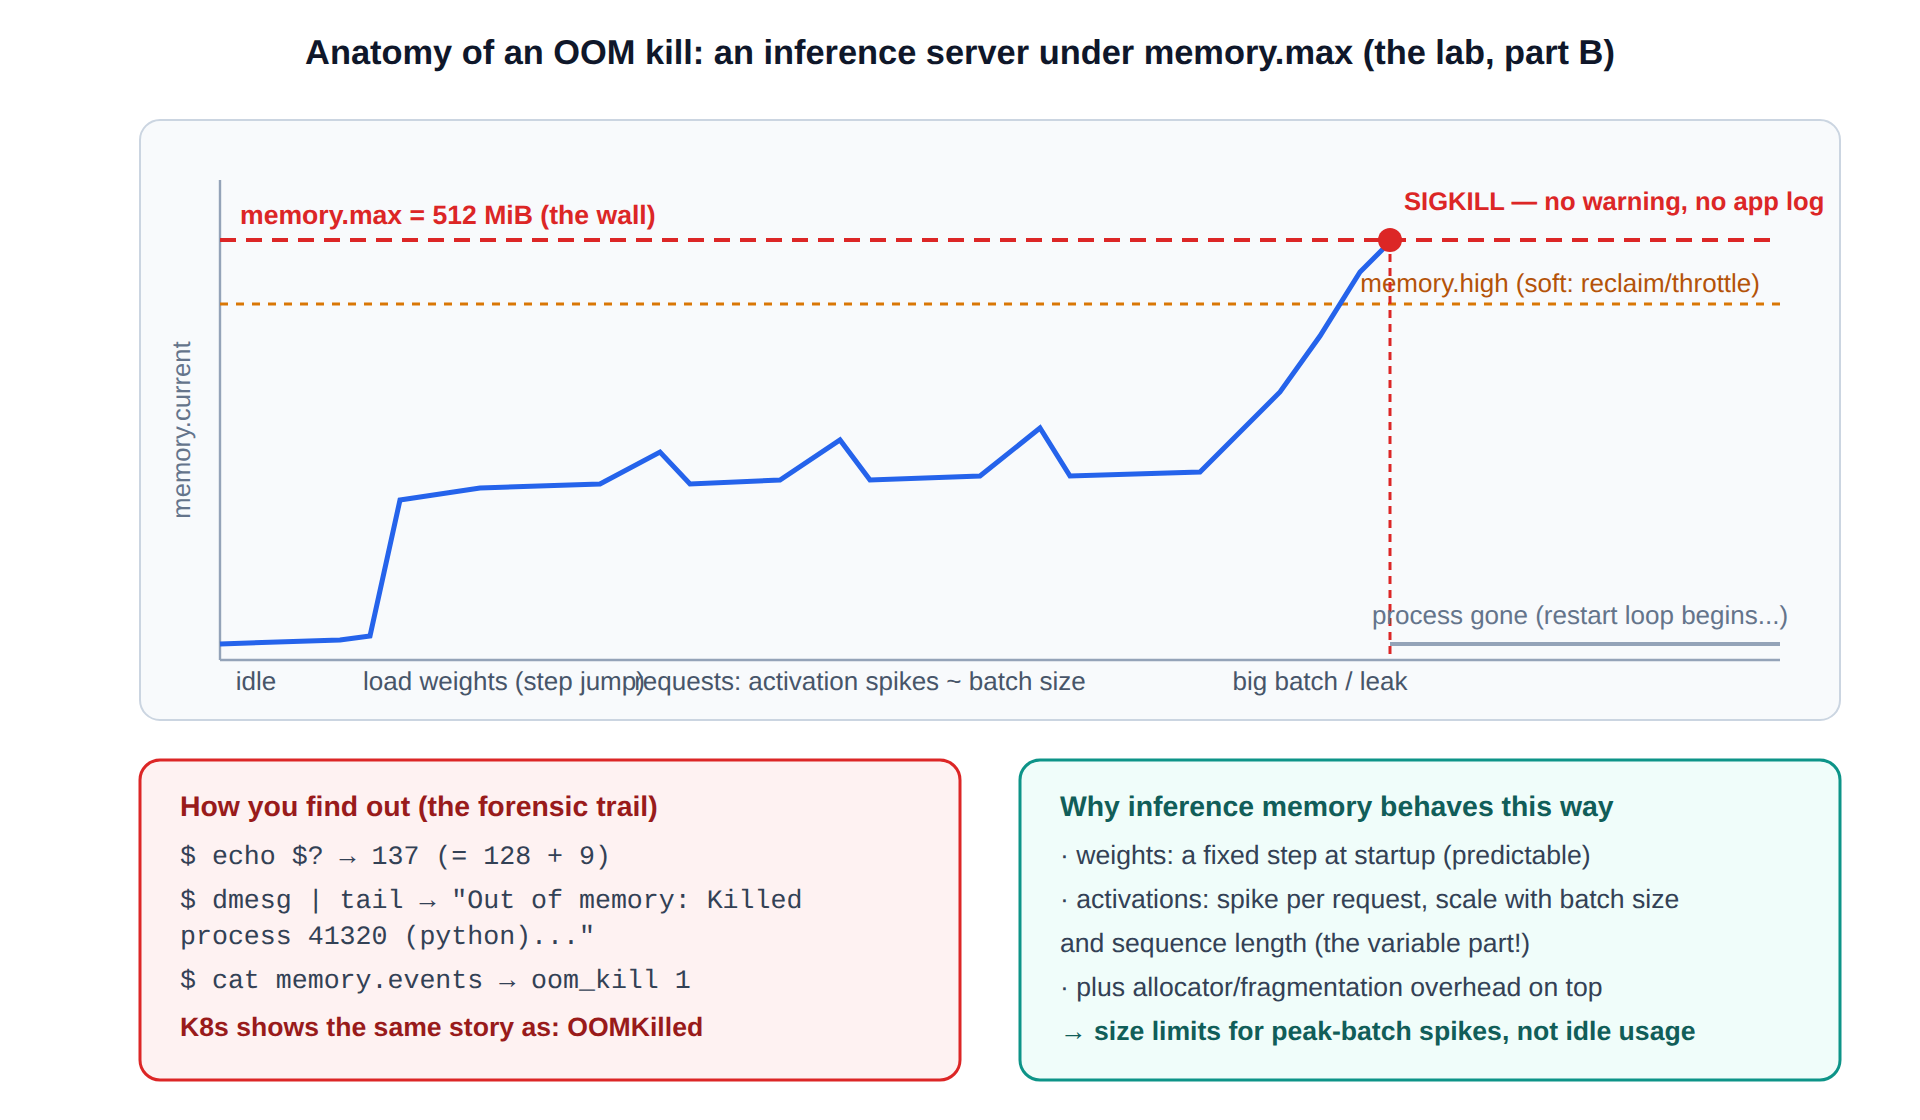
\includegraphics{figures/fig3-7_oom.png}}\\[3pt]
  \figcaption{Figure 3-7  An inference server's memory life under memory.max: the weights step, per-request activation spikes, the fatal crossing, and the forensic trail (137, dmesg, memory.events).}
\end{tbbfigure}

\subsection*{The mechanism, end to end}

Replay Section 3.3's rule as a timeline. The group's \code{memory.current} climbs toward \code{memory.max}; the kernel reclaims what it can — page cache first, which is why file-heavy phases can hug the limit harmlessly; when a new \textbf{anonymous} allocation (heap, tensors) cannot be satisfied even after reclaim, the kernel invokes the \textbf{OOM killer scoped to the cgroup}. It scores the group's processes — essentially by memory footprint, adjustable via \code{oom\_score\_adj} — picks the biggest (in a model server's pod, effectively always the model server), and delivers \textbf{SIGKILL}. SIGKILL cannot be caught, blocked, or handled; there is no cleanup, no flush, no goodbye. The evidence therefore lives entirely \textit{outside} the victim, and you should know each artifact by sight before you need it at 2 a.m.:

\begin{terminalbox}
\begin{Verbatim}[breaklines=true,breakanywhere=true,fontsize=\small,formatcom=\color{tbbtermfg},codes=\tbbcodeactive]
$ echo $?                          # 1) the exit code, wherever the process ran
137                                #    = 128 + 9 (killed by signal 9, SIGKILL)
$ sudo dmesg | grep -i -A1 "out of memory"     # 2) the kernel's confession
Memory cgroup out of memory: Killed process 41320 (python)
  total-vm:1892456kB, anon-rss:498112kB, file-rss:1024kB, ...
$ cat /sys/fs/cgroup/.../memory.events          # 3) the cgroup's ledger
oom 3
oom_kill 1
# 4) and the same story, as Kubernetes tells it (Week 5):
$ kubectl describe pod model-server-7d4b9 | grep -A3 "Last State"
Last State:   Terminated
  Reason:     OOMKilled
  Exit Code:  137
\end{Verbatim}
\end{terminalbox}
\figcaption{Transcript 3-11  The complete OOM evidence chain: exit 137, the dmesg line (note anon-rss — unreclaimable memory — near the limit), the oom\_kill counter, and Kubernetes' echo of all three.}

Note one detail in the \code{dmesg} line that rewards close reading: \code{anon-rss:498112kB} against a 512 MiB limit. The kill happened because \textit{anonymous} memory — the unreclaimable kind — filled the budget; \code{file-rss} (cache-like) is tiny because reclaim had already stripped it. This is Section 3.3's reclaim subtlety, printed by the kernel in its own confession.

\subsection*{Why inference servers, specifically, walk into the wall}

The OOM killer executes the sentence, but the crime is almost always a mis-sized budget — because inference memory has a \textit{shape} that intuition trained on stateless web apps gets wrong. A web handler allocates kilobytes per request around a flat baseline; observed usage ≈ needed usage, and "idle + 10\%" is a fine limit. An inference server is three superimposed curves: a large fixed \textbf{weights} step at startup (predictable, measurable once); a modest steady plateau; and \textbf{per-request activation spikes whose height scales with batch size and sequence length} — the traffic-dependent part — plus allocator overhead (PyTorch's caching allocator holds freed blocks in pools; fragmentation adds more) on top. The plateau tells you almost nothing about the peak.

\begin{calloutbox}{tbbblue}{tbbbluefill}
{\normalsize\bfseries\color{tbbblue}Worked example — sizing memory.max for a small BERT server (lab-scale numbers)}\par\vspace{3pt}
Take a BERT-base classifier served on CPU — roughly the lab's Part B workload. The weights are 110 M parameters × 4 bytes (fp32) ≈ \textbf{440 MB}, loaded once at startup: the step in Figure 3-7. Measured under load (numbers representative of what your lab run will produce):

\begin{tbbitemize}
  \item idle after load: \textbf{\textasciitilde{}620 MB} (weights + runtime + allocator pools)
  \item batch 8 × seq 128: spikes to \textbf{\textasciitilde{}900 MB}  ·  batch 32 × seq 256: spikes to \textbf{\textasciitilde{}1.4 GB}
\end{tbbitemize}

Now compare policies. \textbf{Naive:} limit = idle + 10\% ≈ \textbf{680 MiB} → dies on the \textit{first} batch-8 request; restart loop; each restart re-pays the 440 MB load. \textbf{Peak-sized:} limit = measured worst spike × 1.25 headroom ≈ \textbf{1.75 GiB} → survives everything you load-tested, at the cost of reserving \textasciitilde{}1.1 GB above idle per replica (a density/cost trade, Chapter 1). \textbf{Bounded:} cap serving at batch ≤ 8, seq ≤ 128 in the server config, then limit ≈ 900 MB × 1.25 ≈ \textbf{1.1 GiB} → smaller reservation, bounded worst case — bought by capping throughput (the latency/throughput/cost triangle again). Both non-naive policies are defensible; the naive one is a time bomb with a traffic fuse.
\end{calloutbox}

\vspace{3.0pt}

Two clarifications keep this honest. First, the arithmetic above is the \textit{method}; your numbers will differ — which is exactly why the playbook's first verb is \textbf{measure}, not guess. Second, on GPU serving the same plot runs twice: kernel OOM governs host RAM (this section verbatim), while \textbf{GPU VRAM has a different referee} — exhaustion there raises the CUDA allocator's \code{torch.cuda.OutOfMemoryError}, which \textit{is} catchable in Python (you can shed the request) precisely because it is an allocator error, not a SIGKILL. Distinguishing the two OOMs by their signatures (exit 137 + dmesg vs. a Python traceback) is a genuinely useful diagnostic skill, and Week 11 adds the KV cache as a third, growing character on the VRAM side.

\subsection*{The playbook}

\begin{tbbitemize}
  \item \textbf{Size for peak, not plateau.} Measure \code{memory.current} under a \textit{worst-case load test} — maximum configured batch, longest sequences (Week 9's Locust runs generate exactly this) — and set \code{memory.max} above that peak with explicit headroom (the example used 1.25×). Never derive a limit from idle observation.
  \item \textbf{Bound the variable part.} The spike scales with batch and sequence length; capping both in server config turns unbounded memory behavior into bounded, making the previous step's "worst case" a number that actually exists. This is SLO thinking (Chapter 1) applied to memory.
  \item \textbf{Use memory.high as the tripwire.} Set it below max (the example: high = 1.5 GiB under a 1.75 GiB max) and alarm on \code{memory.events} / pressure signals: you get a graphed warning phase — reclaim, throttling, a climbing counter — instead of a silent execution. Week 14 wires this into dashboards.
  \item \textbf{Read 137 as a diagnosis, not a mystery.} Exit 137 + \code{oom\_kill} in memory.events = budget, not bug. The fix conversation is "resize or bound," never "add try/except" — SIGKILL is uncatchable, and (per the worked example) the fatal allocation is often not even your code's.
  \item \textbf{Know the Kubernetes translation ahead of Week 5:} requests are the scheduler's planning numbers; limits are this chapter's cgroup walls. QoS classes are OOM \textit{priority} policy — Guaranteed pods (requests = limits) get the most protective \code{oom\_score\_adj}, BestEffort pods are first against the wall when a \textit{node} runs short. Swap is typically off in serving clusters: the wall is the wall.
\end{tbbitemize}

\begin{calloutbox}{tbbpurple}{tbbpurplefill}
{\normalsize\bfseries\color{tbbpurple}Think About It}\par\vspace{3pt}
\begin{tbbitemize}
  \item A colleague proposes catching the OOM in Python (try/except MemoryError) for graceful degradation. Using the mechanism and the two-OOMs clarification, explain (a) why it cannot work for the cgroup wall, and (b) where a very similar idea does work on the GPU side.
  \item Your server's measured spikes: 1.9 GB at batch 32, 3.4 GB at batch 64. Node capacity allows 2.5 GiB limits per replica. Using the worked example's method, propose a configuration — and name which corner of the latency/throughput/cost triangle you just traded away.
  \item In Transcript 3-11, suppose dmesg showed file-rss:400000kB and anon-rss:90000kB instead. What would that tell you about the "OOM," and why should the fix differ completely?
\end{tbbitemize}
\end{calloutbox}

\section{Lab: A Mini-Container, and an OOM Observed}

This week's lab has two parts that mirror the chapter's arc: build the box, then hit its wall. Everything runs on any Linux VM or the course cloud instance — no GPU required (and the OOM demonstration is deliberately CPU-only, so no expensive instance is at risk). The handout carries exact commands; this section fixes the intent, the protocol, and the expected observations, so that in the lab you are \textit{confirming} predictions rather than typing blind. Deliverable: a one-page report — transcript highlights and three observations, each tied to a section of this chapter.

\subsection*{Part A — the five moves, performed}

Execute Transcripts 3-8 through 3-10 end to end, capturing four artifacts as you go: the \textbf{hostname contrast} between the two terminals (§3.2's privacy, proven); \textbf{ps showing PID 1 = your shell} after the \code{/\allowbreak proc} mount (§3.2's two truths — and note what \code{ps} printed \textit{before} the mount, because that error message is the "tools read /proc" lesson in the wild); the \textbf{namespace inode comparison} — \code{ls -l /\allowbreak proc/\allowbreak \$\$/\allowbreak ns} inside versus a host shell, confirming every number differs (Transcript 3-2's test, now applied to something you built); and the \textbf{host-side view of your budget} — \code{cat /\allowbreak sys/\allowbreak fs/\allowbreak cgroup/\allowbreak minibox/\allowbreak cgroup.procs} printing the \textit{host} PID of the process your container believes is 1. That last artifact is the chapter's thesis in one line of output: same process, two truths, one budget.

\subsection*{Part B — the execution, observed}

Now the serving lesson. Inside the budgeted container (or a fresh cgroup with \code{memory.max} = 256 MiB), run the handout's toy inference script — it loads a deliberately chunky model object (the weights step), then serves batches of growing size (the activation spikes). Watch from the host in a second terminal:

\begin{terminalbox}
\begin{Verbatim}[breaklines=true,breakanywhere=true,fontsize=\small,formatcom=\color{tbbtermfg},codes=\tbbcodeactive]
# terminal 2 (host): watch the two files that matter, side by side
$ watch -n 0.5 'cat /sys/fs/cgroup/minibox/memory.current \
                 /sys/fs/cgroup/minibox/memory.events'
# you will watch Figure 3-7 draw itself:
#   ~8 MB (idle shell) -> ~120 MB (model loaded) -> spikes with each batch
#   -> at the fatal batch: memory.current snaps DOWN, oom_kill: 0 -> 1
# terminal 1 (container): the victim's-eye view
$ python toy_serve.py
loaded model (112.4 MB)
batch  4 ok   peak ~158 MB
batch 16 ok   peak ~214 MB
Killed                          # <- the shell says this, not Python
$ echo $?
137
\end{Verbatim}
\end{terminalbox}
\figcaption{Transcript 3-12  Part B, as it should unfold. Note who says "Killed" — the shell, reporting the signal; Python never gets a last word. Then collect dmesg and memory.events per Transcript 3-11.}

Then run the two follow-ups that turn observation into engineering: \textbf{(1)} set \code{memory.high} to 200 MiB and repeat — you will see the pre-wall phase change character (progress slows, reclaim churns, \code{memory.events} counts pressure) before any kill: your tripwire experience, and a preview of what a good Week 14 alert fires on; \textbf{(2)} cap the script's batch size at the largest value that survived, and demonstrate the same 256 MiB limit now survives the full run — the "bound the variable part" fix, proven by you, with the worked example's method now backed by your own numbers.

\begin{calloutbox}{tbbpurple}{tbbpurplefill}
{\normalsize\bfseries\color{tbbpurple}Lab checklist}\par\vspace{3pt}
\begin{tbbitemize}
  \item Part A artifacts: hostname contrast · ps before/after the /proc mount · /proc/\$\$/ns inside vs. outside · host-side cgroup.procs.
  \item Part B artifacts: memory.current timeline (even hand-noted) · exit code 137 · dmesg line (quote the anon-rss figure) · memory.events counter.
  \item Follow-ups: memory.high warning-phase behavior · batch-cap rerun surviving the same limit.
  \item Report: three observations, each naming its section (e.g., "ps failed before the proc mount — §3.2's tools-read-/proc lesson").
  \item Cleanup: exit the shell, rmdir the cgroup, delete the rootfs. (No cloud meter this week — but keep the Chapter 2 habit.)
\end{tbbitemize}
\end{calloutbox}

\vspace{3.0pt}

\begin{calloutbox}{tbbpurple}{tbbpurplefill}
{\normalsize\bfseries\color{tbbpurple}Think About It}\par\vspace{3pt}
\begin{tbbitemize}
  \item During Part B, memory.current sometimes drops on its own before the kill. What is the kernel doing, which §3.3 subtlety does it illustrate, and why does it delay but not prevent the OOM here?
  \item Predict before running: if the toy server forks two workers and the fatal spike happens in a worker, which process does the OOM killer take — and what does your server look like afterward? (oom\_score is the hint; verify in the lab, then connect to why tini's reaping duty matters.)
\end{tbbitemize}
\end{calloutbox}

\namedsection{Summary}{The Chapter in Ten Points}

\qitem{1}{\textbf{There is no container object in the kernel.} A container is a convention: namespaces (what a process sees) + cgroups (what it may use) + a layered filesystem (where its world comes from), wrapped around an ordinary process on a shared kernel — Chapter 2's isolation-spectrum caveat, now mechanistic.}

\qitem{2}{\textbf{Namespaces privatize views}, not machines: PID, NET, MNT, UTS, IPC, USER (plus cgroup and time). The API is unshare/clone/setns — and \code{docker exec} is just setns in a trench coat.}

\qitem{3}{\textbf{PID 1 is a job}: reap orphans, handle signals — or rollouts end in SIGKILL after ignored SIGTERMs. Handle SIGTERM in your server or run tini. This one paragraph prevents real incidents.}

\qitem{4}{\textbf{NET namespaces give every container its own port space}, wired out by veth pairs into a host bridge with NAT. A Kubernetes pod = containers sharing one NET namespace — hence localhost sidecars and one-IP-per-pod (Week 5).}

\qitem{5}{\textbf{cgroups v2 is a filesystem of budgets}: echo limits into files, enroll PIDs, read usage back. Docker flags and K8s limits are ghostwriters for these files.}

\qitem{6}{\textbf{cpu.max throttles in bursts} — a process pauses, wholesale, when its window quota is spent. Invisible to profilers, visible in cpu.stat's nr\_throttled, lethal to p99. Cousin of Chapter 2's steal time.}

\qitem{7}{\textbf{memory.max is a wall with an enforcer.} Cross it after failed reclaim and the OOM killer SIGKILLs the biggest process in the cgroup: exit 137, dmesg confession, memory.events oom\_kill, K8s "OOMKilled". Not an error path — the enforcement of a budget you chose.}

\qitem{8}{\textbf{Inference memory is a step + plateau + traffic-scaled spikes} (weights, then batch/sequence-dependent activations). Size limits for measured peak, bound batch/length, tripwire with memory.high — never size to idle.}

\qitem{9}{\textbf{overlayfs makes images economical}: read-only layers shared host-wide, one thin writable upper per container, copy-up on write, whiteouts on delete. Layer-by-rate-of-change ⇒ dedup, build cache, instant filesystem start — and image pulls as the true cold-start cost (Week 12). Weights belong in the model store, not layers.}

\qitem{10}{\textbf{You can build a container by hand in five moves} — unshare, hostname, pivot\_root, mount /proc, cgroup — and therefore know exactly what Docker adds: images/registries, network defaults, lifecycle API, and the standardized runtime split (containerd/runc/OCI) that is Week 4's subject, GPU access included.}

\namedsection{Exercises}{}

\subsection*{A. Multiple choice}

\qitem{1}{Which statement about containers and the Linux kernel is correct?}

\begin{tbboptions}
  \item ① The kernel provides a container object created by a dedicated syscall
  \item ② A container is a kernel-scheduled ordinary process wrapped in namespaces, cgroups, and a mounted layered filesystem
  \item ③ Containers run a second kernel, like lightweight VMs
  \item ④ Containers are a Docker-proprietary kernel feature
\end{tbboptions}

\qitem{2}{A containerized server ignores SIGTERM during rollouts and is SIGKILLed after the grace period. The most likely cause is:}

\begin{tbboptions}
  \item ① The NET namespace drops signals from outside
  \item ② cgroups block signal delivery when CPU-throttled
  \item ③ The server runs as PID 1 in its PID namespace and never installed a SIGTERM handler — PID 1 gets no default dispositions
  \item ④ overlayfs made the process read-only
\end{tbboptions}

\qitem{3}{cpu.max is set to "25000 100000" for an inference container. Which observation is most consistent with that setting under load?}

\begin{tbboptions}
  \item ① All requests uniformly 4× slower
  \item ② p50 barely moves, but p99 grows spikes up to \textasciitilde{}75 ms while cpu.stat's nr\_throttled climbs
  \item ③ The container is killed with exit 137
  \item ④ Nothing — cpu.max only affects batch jobs
\end{tbboptions}

\qitem{4}{A pod dies with exit code 137, no application logs, and memory.events shows oom\_kill: 1. The correct first interpretation is:}

\begin{tbboptions}
  \item ① A segfault in the model runtime — file a bug upstream
  \item ② The kernel enforced memory.max: reclaim failed, the OOM killer SIGKILLed the largest process in the cgroup
  \item ③ The image was corrupted during pull
  \item ④ Kubernetes evicted the pod for low disk
\end{tbboptions}

\qitem{5}{Thirty containers on one node all use the same 8 GB PyTorch base image. Approximate additional disk for the 30th container's filesystem:}

\begin{tbboptions}
  \item ① \textasciitilde{}8 GB — each container copies the image
  \item ② \textasciitilde{}4 GB — copy-on-write halves it
  \item ③ \textasciitilde{}0 — layers are shared read-only; each container adds only a thin writable upper dir
  \item ④ It depends on memory.max
\end{tbboptions}

\qitem{6}{Why do real container runtimes use pivot\_root rather than chroot for the private root?}

\begin{tbboptions}
  \item ① pivot\_root is faster at file I/O
  \item ② chroot cannot be used inside namespaces
  \item ③ pivot\_root actually replaces the mount namespace's root and detaches the old one; chroot merely repoints a path and is escapable by design
  \item ④ pivot\_root compresses the rootfs
\end{tbboptions}

\subsection*{B. Short answer}

\qitem{1}{Name the three ingredients of the container recipe and the one-phrase job of each.}

\qitem{2}{Decode exit code 137 arithmetically, and name the two places outside the process where the OOM kill leaves evidence.}

\qitem{3}{A Kubernetes pod's two containers talk over localhost. Which namespace must they share for that to work, and what pod property follows from it?}

\qitem{4}{Your Dockerfile step \code{RUN rm -rf /\allowbreak opt/\allowbreak samples} (in its own layer) fails to shrink the image. Name the overlayfs mechanism responsible, in one sentence.}

\subsection*{C. Essay}

\qitem{1}{Walk through the five moves of building a container by hand (§3.5), stating for each move which chapter mechanism it exercises and what observable proof you would capture that it worked. Conclude with two things Docker adds that your hand-built container lacks.}

\qitem{2}{An inference pod (limit 2 GiB) OOM-kills roughly daily, always near traffic peaks. Idle usage is 1.1 GiB. Write the diagnosis and a remediation plan using §3.6's playbook: what you would measure, how you would resize or bound, which tripwire you would set, and what trade-off (Chapter 1 vocabulary) each step makes.}

\qitem{3}{"Containers won because of overlayfs, not namespaces." Argue for and against this claim, using the economics of §3.4 (dedup, cache, startup, distribution) versus the isolation and operational properties of §3.2–3.3. Take a final position and defend it in terms relevant to serving systems.}

\namedsection{Answers and Commentary}{}

\subsection*{A. Multiple choice}

\qitem{1}{\textbf{②} The recipe view. No kernel container object exists (①), no second kernel is involved — that is Chapter 2's VM (③), and the mechanisms are vendor-neutral kernel features (④). (§3.1)}

\qitem{2}{\textbf{③} PID 1 semantics: the kernel disables default signal dispositions for init, so an unhandled SIGTERM is ignored rather than fatal. Fix in code or with tini/--init. (§3.2)}

\qitem{3}{\textbf{②} "25000 100000" = 25 ms per 100 ms window: bursts of full speed, then enforced pauses up to 75 ms — classic throttling tail-latency, confirmed by nr\_throttled. 137 (③) is memory's signature, not CPU's. (§3.3)}

\qitem{4}{\textbf{②} That triple — 137, silent app, oom\_kill counter — is the OOM evidence chain verbatim. The conversation is "resize or bound the budget," not "debug a crash." (§3.6)}

\qitem{5}{\textbf{③} Layers are shared read-only host-wide; per-container cost is the near-empty upperdir. This is the dedup economics that makes multi-GB ML images workable. (§3.4)}

\qitem{6}{\textbf{③} pivot\_root swaps the mount namespace's root and lets you unmount the old world; chroot leaves it reachable (the classic escape) — demo shortcut vs. production mechanism. (§3.5)}

\subsection*{B. Short answer}

\qitem{1}{\textbf{Namespaces} — privatize what the process sees; \textbf{cgroups v2} — bound what it uses; \textbf{overlayfs (+ pivot\_root)} — supply its root filesystem from shared read-only layers.}

\qitem{2}{137 = 128 + 9, i.e., death by signal 9 (SIGKILL). Evidence: host \code{dmesg} ("Out of memory: Killed process ...") and the cgroup's \code{memory.events} (\code{oom\_kill} counter) — plus K8s's \code{OOMKilled} status as the platform echo.}

\qitem{3}{The \textbf{NET namespace}. Sharing it gives all pod containers one network stack — hence one IP per pod and sidecars on localhost. (They keep separate MNT namespaces — different filesystems.)}

\qitem{4}{\textbf{Whiteout semantics}: a later layer can only \textit{hide} files from lower read-only layers, not remove their bytes; the deleted content still ships in the earlier layer.}

\subsection*{C. Essay (grading points)}

\qitem{1}{Look for: unshare (namespaces §3.2; proof: /proc/\$\$/ns inodes differ) → hostname (UTS; proof: inside/outside contrast) → pivot\_root over an unpacked rootfs (MNT + §3.4; proof: private /) → mount /proc (proof: ps shows PID 1 — and the meta-lesson that tools read /proc) → cgroup enrollment (§3.3; proof: cgroup.procs shows the host PID). Docker adds (any two): images/registries, network wiring, lifecycle API/daemon, OCI runtime split. Full credit requires proofs, not just commands. (§3.5)}

\qitem{2}{Diagnosis: limit sized near plateau (1.1 GiB idle) while spikes scale with batch/sequence — peak-time deaths are the §3.6 signature. Plan: load-test at max batch/length while recording memory.current peak (Week 9 tooling); either raise limit above measured peak + headroom (trade: fewer replicas per node — a cost/utilization trade, Ch. 1) or cap batch/sequence (trade: throughput ceiling — the latency/throughput tension); set memory.high tripwire + alert on memory.events; re-verify under the same load test. Bonus: mention that restart loops also pay the model-load cold start, compounding user impact. (§3.6)}

\qitem{3}{A good "for" argues distribution economics: layers made multi-GB environments shippable, cacheable, dense, and fast to start — without which namespace tech would have remained a sysadmin curiosity (and cgroups predate Docker's rise). A good "against" argues that ports, PID trees, and resource walls are what make co-tenancy \textit{safe enough to want} — density without isolation is just a shared box. Either final position earns full credit if it engages serving specifics: image-pull cold starts and layer hygiene (for), OOM walls and port privacy for replica fleets (against). (§3.2–3.4)}

\namedsection{Further Reading}{}

Entries tagged \textbf{[This week]} are required viewing or reading now; a \textbf{[Wk N]} tag marks material that pays off in that later week.

\begin{tbbitemize}
  \item \textbf{[This week] Liz Rice, "Containers from Scratch" (GOTO 2018, video)} — this week's required viewing and the lab's original. A container built live in a few dozen lines of Go. Watch it \textit{after} attempting Part A yourself: the déjà vu is the point.
  \item \textbf{[This week] man pages: namespaces(7), cgroups(7), unshare(1), pivot\_root(2)} — unusually well-written for kernel documentation, and the authoritative details behind §3.2–3.3. Read namespaces(7) in full once; skim the rest as lab support.
  \item \textbf{Liz Rice, "Container Security" (O'Reilly, 2020)} — the book-length version of this chapter's worldview: chapters 2–6 cover namespaces, cgroups, and image layers with a security lens that complements our serving lens.
  \item \textbf{The cgroup v2 kernel documentation (admin-guide/cgroup-v2)} — the primary source for controller semantics; the memory-controller section reads as a commentary on §3.6. Pair with LWN's cgroup v2 series for the design history.
  \item \textbf{Docker docs: "About storage drivers" and "Use the OverlayFS storage driver"} — concrete, well-diagrammed treatment of layers, copy-up, and whiteouts; the practical companion to §3.4.
  \item \textbf{[Wk 4] OCI Runtime Specification} (opencontainers.org) — skim config.json once now: you will recognize every field (namespaces, cgroups, mounts, root) as this chapter in JSON. It becomes central in Week 4.
  \item \textbf{[Wk 5] Kubernetes docs: "Resource Management for Pods and Containers"} — read after Week 5's chapter; you will now see requests/limits as scheduler inputs vs. cgroup writes, and QoS classes as OOM-priority policy.
  \item \textbf{[Wk 4] NVIDIA Container Toolkit documentation} — next week's bridge: how a GPU device, driver libraries, and CUDA runtime get injected into the box you built this week.
\end{tbbitemize}

\vspace{5.0pt}

\begin{calloutbox}{tbbblue}{tbbbluefill}
{\normalsize\bfseries\color{tbbblue}Next chapter — Chapter 4: Docker and the Container Runtime Stack}\par\vspace{3pt}
You can now build a container with your hands — next week we meet the industrial machinery that does it a billion times a day. How the pieces are organized (Docker → containerd → runc) and why the OCI specifications make runtimes swappable (recall Kata and gVisor slotting under Kubernetes); how images are built well (Dockerfile layer discipline, multi-stage builds — §3.4 turned into engineering practice) and moved (registries, digests, pulls — your cold-start line item); and the question this course has been saving: \textbf{how does a GPU get into the box?} The NVIDIA Container Toolkit, device injection, and why "cgroups can't schedule GPU compute" (§3.3) shapes everything about ML containers. Lab: containerize the FastAPI model server from Week 1's stack diagram and push it to a registry — the image you will deploy to Kubernetes in Week 5.
\end{calloutbox}
